\documentclass[12pt]{cheatsheet}
\usepackage{blindtext}
\usepackage{enumitem}
\usepackage{amsmath}
\usepackage{xcolor}
\usepackage{cancel}

\author{Gian Maria Ernst :)) - ernstg\\  \vspace*{0.2em} \normalsize{Based on the work by F. Spengler} \vspace*{-0.2em}}\doctitle{Fertigunstechnik}

\begin{document}
\small

\section*{Definition und Aufgaben}
    \textbf{Definition:}
\begin{itemize}
    \item Reproduzierbare Umwandlung von Rohstoffen zu Produkten
    \item Herstellung Geometrisch bestimmter fester Körper
\end{itemize}

\textbf{Aufgaben:}
\begin{itemize}
    \item Erzeugung eines Mehrwerts
    \item Minimierung der Energie, Fertigungsschritte und Umweltbelastung
    \item Auswahl geeigneter Werkstoffe und Fertigungsverfahren
\end{itemize}

\textbf{NC-Programmiersysteme:}
\begin{itemize}
    \item Programmierunterstützung beim Drehen, Fräsen, Bohren
    \item Automatische Dimensionierung von Bauteilen
    \item Automatische Schnittaufteilung
\end{itemize}

\section*{Kostenrechnung}
    \subsection*{Maschinenstundensatz}
    \begin{tiny}
\[
\boxed{
    \begin{aligned}
        \textcolor{red} {K_{MH}} &= \frac{\textcolor{blue}{K_A} + \textcolor{green}{K_Z} + \textcolor{violet}{K_R} + K_I + K_E}{\textcolor{cyan}{T_L}} \\
        \textcolor{cyan}{T_L} &= x_s \cdot x_d \cdot x_j \cdot x_N
    \end{aligned}
}
\]

\begin{minipage}{0.53\linewidth}
    \item $\textcolor{red} {K_{MH}}$: Maschinenstundensatz $\left[\$\text{/h}\right]$
    \item $\textcolor{blue}{K_A}$ : Abschreibungskosten $\left[\$\text{/j}\right]$
    \item $\textcolor{green}{K_Z}$ : Zinsen $\left[\$\text{/j}\right]$
    \item $\textcolor{violet}{K_R}$ : Reparaturkosten $\left[\$\text{/j}\right]$
    \item $K_I$ : Instandhaltungskosten $\left[\$\text{/j}\right]$
    \item $K_E$ : Energiekosten $\left[\$\text{/j}\right]$
\end{minipage}
\begin{minipage}{0.46\linewidth}
    \item $\textcolor{cyan}{T_L}$ : Nutzungsdauer $\left[\text{h/j}\right]$
    \item $x_s$ : \# Schichten 
    \item $x_d$ : Schichtdauer $\left[\text{h/d}\right]$
    \item $x_j$ : Jahresarbeitstage $\left[\text{d/j}\right]$
    \item $x_N$ : Nutzungsgrad
\end{minipage}
\vspace{1mm}

\[
\boxed{
    \begin{aligned}
        \textcolor{blue}{K_A} = \frac{WBW}{T_N}, 
        \textcolor{green}{K_Z} = \frac{AW + RW}{2} \cdot x_Z, 
        \textcolor{violet}{K_R} = w \cdot F
    \end{aligned}
}
\]

\begin{minipage}{0.45\linewidth}
    \item $WBW$: Wiederbeschaffungswert d. Maschine $\left[\$\right]$
    \item $T_N$: Gesamtnutzungsdauer $\left[\text{a}\right]$
    \item $AW$: Anschaffungswert $\left[\$\right]$
    \item $RW$: Restwert $\left[\$\right]$
    \item $x_Z$: kalk. Zinssatz $\left[1\text{/a}\right]$
\end{minipage}
\begin{minipage}{0.55\linewidth}
    \item $w$: Raumkosten pro Fläche $\left[\frac{\$}{\text{a} \cdot \text{m}^2}\right]$
    \item $F$: Grundfläche der Anlage $\left[\text{m}^2\right]$
\end{minipage}
\vspace{1mm}
\end{tiny}
    \subsection*{Stückkosten}
    \begin{tiny}
\begin{center}
    Stückkosten $k$ = Variable Kosten $k_V$ + fixe Kosten $k_F$   
\end{center}
\vspace{1mm}

\begin{minipage}{0.5\linewidth}
    \begin{footnotesize}
        \begin{center}
            \mathbox{
                K_{VO} = K_S + K_{PR}
            }
        \end{center}
    \end{footnotesize}
\end{minipage}
\begin{minipage}{0.5\linewidth}
        \item $K_{VO}$: Vorbereitungskosten $\left[\$\right]$
        \item $K_S$: Wekzeug und Messkosten $\left[\$\right]$
        \item $K_{PR}$: Prüfkosten $\left[\$\right]$
\end{minipage}
\vspace{1mm}

\hspace{0.05\linewidth}

\begin{minipage}{0.5\linewidth}
\[
\boxed{
    \begin{aligned}
        K_{AW} = (&\textcolor{red} {K_{MH}} + \textcolor{teal}{K_{LH}}) \cdot t_R\\
        &+ K_{RA} + K_T
    \end{aligned}
}
\]
\end{minipage}
\begin{minipage}{0.5\linewidth}
        \item $K_{AW}$: Auftr.wiederholkosten $\left[\$\right]$
        \item $\textcolor{teal}{K_{LH}}$: Lohnkosten $\left[\$\right]$
        \item $t_R$: Rüstzeit $\left[\text{h}\right]$
        \item $K_{RA}$: Rüstkosten $\left[\$\right]$
        \item $K_T$: Fertigungssteuerung $\left[\$\right]$
\end{minipage}
\vspace{1mm}

\hspace{0.05\linewidth}

\begin{minipage}{0.5\linewidth}
    \[
    \boxed{        
        \begin{aligned}
            K_{FE} = (&\textcolor{red} {K_{MH}} + \textcolor{teal}{K_{LH}} \\
            &+ K_{WH}) \cdot t_e
        \end{aligned}
    }
    \]
    \end{minipage}
    \begin{minipage}{0.5\linewidth}
            \item $K_{FE}$: Fertigungskosten $\left[\$\right]$
            \item $K_{WH}$: Werkzeugkosten $\left[\$\right]$
            \item $t_e$: Fertigungszeit $\left[\text{h}\right]$
    \end{minipage}
    \vspace{1mm}
\end{tiny}


    \vfill \null \columnbreak

\section*{Prozesse und Prozessketten}
    \textbf{Planungsprozesse:}\\
\textbf{Key Performance Dimensions:} Vorlaufzeit$\downarrow$ , Qualität $\uparrow $, Emissionen $\downarrow $, Kosten $\downarrow $\\
\textbf{Concurrent engineering:} Ermöglicht gleichzeitige Arbeitsschritte (nicht seq./ nicht lin.). \\
\textbf{CAE:} Computer Aided Engineering \\
\textbf{CAM:} Computer Aided Manufacturing \\
\textbf{Lean Manufacturing:} Kosten $\downarrow$ und Produktivität $\uparrow $\\
Fünf Prinzipien: Definition des Wertes für Kunden, Identifikation des Wertstroms, \\Umsetzung des Flussprinzips, Einführung des Pull-Prinzips, Streben nach Perfektion. \\
\textbf{Verschwendung:} Überproduktion, Unnötige Bewegung, Hohe Bestände, Transport, Wartezeiten, Ineffizienz, Nacharbeit/Ausschuss.\\
\textbf{Kanban:} "Visuelle Karte". Klassisches Pull-System. Selbstregulierende Regelkreise gewährleiten Materialversorgung. Es wird alles nur auf Nachfrage ausgeführt. Verhindern von Überproduktion. \\
\textbf{Automatisierungspyramide:} Feldebene (Sensoren \& Aktoren), Steuerungsebene (Steuerungen und Überwachungsanlagen), Leitebene (Erfasst und Daten und zeigt diese an), Unternehmensebene (Regelt und steuert die ganzen Systeme).\\


\textbf{Prozesse:}
\begin{itemize}
    \item Urformen  (Gießen, Sintern, 3D)
    \item Umformen  (Schmieden, Walzen, Tiefziehen)
    \item Trennen (Drehen, Fräsen, Bohren, Scherschneiden)
    \item Fügen (Schweissen, Löten, Kleben)
    \item Beschichten  (Galvanisieren, Lackieren, Aufdampfen)
    \item Stoffeigenschaften ändern  (Härten, Glühen, Magnetisieren)
\end{itemize}
\hspace{0.05\linewidth}


    \textbf{Messen und Prüfen:}
\begin{itemize}
    \item Messen: Quantitative und vergleichende Erfassung einer Eigenschaft
    \\Ermitteln einer Länge/ Winkel mit einem Messgerät $\rightarrow$ Messwert
    \item Prüfen: Qualitative Beurteilung einer gemessenen Eigenschaft
    \\Prüfen ob Gegenstand die geforderten Merkmale aufweist $\rightarrow$ Funktionstüchtig
    \item Kalibrieren: Vergleich eines Messwertes mit dem genormten Referenzstandart,
    Dokumentieren der Abweichung, Berechnung der Messunsicherheit und Erstellen des Zertifikates.
\end{itemize}
\hspace{0.05\linewidth}

\textbf{Berührende Messverfahren:}\\
Geometrie der Tastspitze beeinflusst 
gemessene Rauheit. Empfindliche Oberflächen können durch die Berührung der Tastspitze 
beschädigt werden. Flächige Messung nur mit hohem Aufwand 
(Messzeit) realisierbar.\\

\textbf{Optische Messverfahren:}\\
Hohe Messgeschwindigkeit. Schwierigkeiten bei spiegelnden 
Oberflächen. Oberfläche muss sauber sein\\

\textbf{Messunsicherheiten} entstehen durch: Vibrationen, elektromagnetische 
Felder, Staub und Temperaturschwankungen.


    \subsection*{Prozessfähigkeit}
    \textbf{Prozessfähigkeitsindex $C_p$:} 
\begin{itemize}
    \item Verhältnis der Toleranzbreite zur Streuung der Prozesswerte
    \item Ignoriert Lage der Prozesswerte
    \item Kann der Prozess innerhalb der Toleranzen bleiben, wenn er perfekt zentriert ist?
\end{itemize}
\hspace{0.05\linewidth}
\vfill \null \columnbreak

\textbf{Prozessfähigkeitsindex mit Lagekorrektur $C_{pk}$:}
\begin{itemize}
    \item Berücksichtigt auch die Lage der Prozesswerte
    \item Tatsächliche Prozessfähigkeit
    \item Wie gut arbeitet der Prozess tatsächlich?
\end{itemize}
\hspace{0.05\linewidth}

\begin{center}
    $C_p = \frac{OTG - UTG}{6\sigma}$ \hspace{1cm}
    $C_{pk} = \frac{\min\left(OTG - \mu, \mu - UTG\right)}{3\sigma}$
\end{center}
\hspace{0.05\linewidth}

\begin{minipage}{0.7\linewidth
    }
    \begin{itemize}
        \item $C < 1 $: Prozess kann Spezifikationen nicht erfüllen
        \item $C = 1 $: Prozess bedingt geeinget
        \item $C > 1 $: Prozess kann Spezifikationen erfüllen
    \end{itemize}
\end{minipage}
\vspace{1mm}
\hspace{0.05\linewidth}

    \subsection*{Rauheiten}
    
\includegraphics[width = 60mm]{src/images/rauheiten.png}
\item $\mathbf{R_{z}}$: gemittelte Rautiefe – Mittelwert zwischen höchstem und tiefstem Punkt aus 5 aufeinanderfolgenden Intervallen
\item $\mathbf{R_{max}}$: maximale Rautiefe – grösste Differenz inerhalb eines Intervalls
\item $\mathbf{R_{t}}$: Gesamthöhe des Profils – grösste Differenz über die gesamte Länge
\item $\mathbf{R_{a}}$: arithmetischer Mittelwert – Mittelwert der absoluten Profilwerte
\item $\mathbf{R_{q}}$: Quadratischer Mittelwert – gewichtet grosse Werte stärker
\begin{center}
    $\mathbf{R_{t} > R_{max} > R_{z}}$ \hspace{1cm}
    $\mathbf{R_{a} > R_{q}}$
\end{center}

    \subsection*{Lagetoleranzen}
    \includegraphics[width = 40mm]{src/images/lagetoleranzen.png}
    \subsection*{Gestaltabweichungen}
    \begin{itemize}
    \item 1 Ord. Form - Gerad, Eben, Rundheitsabweichung
    \item 2 Ord. Welligkeit - Wellen
    \item 3 Ord. Rauheit - Rillen
    \item 4 Ord. Rauheit - Riefen, Schuppen, Kuppen
    \item 5 Ord. Gefügestruktur
    \item 6 Ord. Gitterfehler
\end{itemize}

\section*{Simulation}
    \textbf{Ziele:}\\
Entwicklungszeit $\downarrow$, Fehler $\downarrow$, Fertigungsverfahren planen, 
Fertigung optimieren, Ausschuss $\downarrow $, Zusammenhänge 
verstehen und vorhersehen, Kosten planen\\

\textbf{Typen:}
\begin{itemize}
    \item Analytische/nichtumerische Simulation (CFD, FEM)
    \item Grafische Simulation (CAD, VR)
    \item Realexperimente
\end{itemize}
\hspace{0.05\linewidth}

\textbf{Möglichkeiten:}\\
Giessprozesse (Formfüllung Erstarrung), Umformen (Kraft, Spannungen, Mikrostruktur), Zerspanung (Spanbildung, Thermik), Fügen (Schweissnähte, Verzug, Einflusszone), Werkstoffe (mikrostruktur, Gefüge, Kristalle) \\

\textbf{Schritte zur FE Lösung:}\\
Zu lösendes Problem $\rightarrow$ Variationsformulierung $\rightarrow$ Diskretisierung $\rightarrow$ Assemblierung\\ $\rightarrow$ Lösung der DGL\\
%\vfill \null \columnbreak

\textbf{Wahre vs FEM Lösung:}\\
Im FEM wird nur an endlich vielen Punkten gerechnet. Mit der FEM-Lösung wird die ursprüngliche DGL nicht notwendigerweise exakt erfüllt. \\

\textbf{Fehlerquellen:} 
Phsikalisches System, Mathematisches Modell, Diskretes Modell, FEM Lösung \\

Die \textbf{Analytische} Lösung erfüllt Feldproblem auf gesamten Lösungsgebiet.

Für \textbf{FEM bei thermischen Problemen} werden drei unabhängige Kennwerte (Wärmekapazität $c$, Wärmeleitfähigkeit $\lambda$, Dichte $\rho$) benötigt.\\

\textbf{1D Wärmeleitung mit FEM:} $\frac{\partial T}{\partial t} = - \frac{k}{c_p \rho }\Delta T$

\subsection*{Nichtlinearitäten:}
bei \textbf{grossen Deformationen}, \textbf{Reibung} und \textbf{Zeitabhängigkeit}\\
Die Lösung ist dann nicht in einem Schritt möglich, sondern via Iteration (Zeitdiskretisierung).\\ 

Es gibt drei Arten von Nichtlinearitäten:
\begin{itemize}
    \item Geometrisch: Verformung zu gross
    \item Materialbasiert: nichtlineares Materialverhalten
    \item Strukturbasiert: Lagerbedingungen verändern sich
\end{itemize}
Bei Zerspanung treten alle drei auf.

\subsection{Implizite vs. explizite FEM}

\textbf{Implizit:} \\
\begin{minipage}{0.45\linewidth}
    \begin{plusitemize}
        \item Grössere Zeitschritte möglich 
        \item stabiles Verfahren falls Konvergenz
        \item Effektiv bei kleinen, linearen und statischen Problemen
    \end{plusitemize}
\end{minipage}
\begin{minipage}{0.5\linewidth}
    \begin{minusitemize}
        \item Hoher Zeitaufwand 
        \item Keine Konvergenz bei Instabilitäten (Beulen oder Falten)
    \end{minusitemize}
\end{minipage}
\\

\textbf{Explizit:} \\
\begin{minipage}{0.45\linewidth}
    \begin{plusitemize}
        \item Gut für hochdynamische, grosse Systeme
        \item Gut bei Nichtlinearitäten
        \item Sehr effektiv bei diagonaler Massematrix 
        \item schnellere Konvergenz
    \end{plusitemize}
\end{minipage}
\begin{minipage}{0.5\linewidth}
    \begin{minusitemize}
        \item kleinere Zeitschritte
        \item Bedingt stabil
        \item Skalierung von Masse oder Zeit führt zu dynamischen Effekten
        \item numerische Fehler schwer abschätzbar
    \end{minusitemize}
\end{minipage}

    \vfill \null \columnbreak


\section*{Urformen}
    \subsection*{Giessystem}
    
\begin{minipage}{0.5\linewidth}
    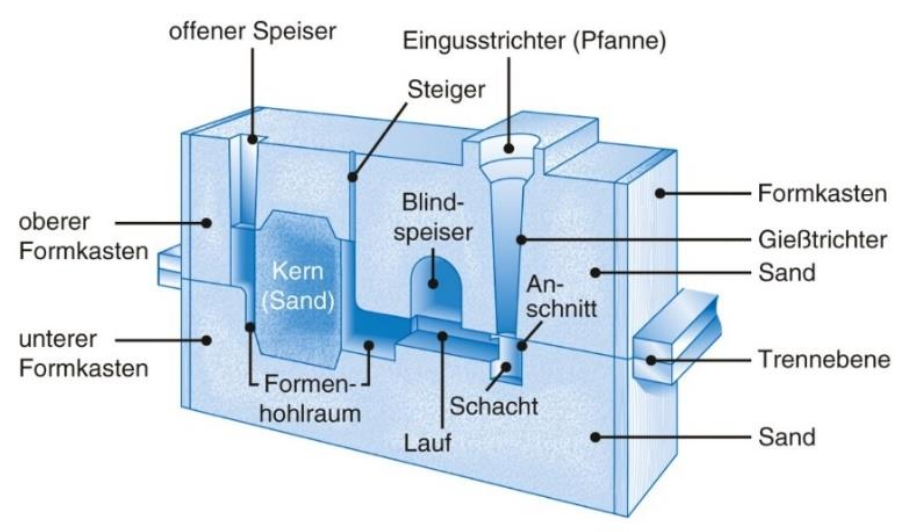
\includegraphics[width = 40mm]{src/images/Giesssystem.png}
\end{minipage}
    \begin{minipage}{0.5\linewidth}
        \begin{itemize}
            \item Anschnitt: System der Zuleitungen.
            Dient zur Steuerung von Füll- und Erstarrungs-
            vorgang, sowie zum Auffangen von Verunreini-
            gungen.
            \item Speiser: Reservebehälter für Schmelze, die in
            die Hohlräume nachfliesst, um Schwindung
            auszugleichen. \\
            Verhältnis von Volumen zu Ober-
            fläche sollte grösser sein als beim Gussstück.
        \end{itemize}
    \end{minipage}
    \vspace{1mm}
    
    \subsection*{Verlorene Formen}
    \textbf{Sandguss} in Formsand ist mengenmässig vorherrschend.\\

\textbf{Lost-Foam Giessen} oder \textbf{Vollformgiessen} ist sehr gut für komplexe Bauteile.\\
Dabei werden Schäumlinge in Sand eingebettet. \\
Vorteile: hohe Bauteilkomplexität, geringe Nachbearbeitung und hohe Automation.\\
Nachteile: hohe Anforderungen an Modellqualität, Zersetzung des Schaums in giftige Gase, Wandsärken $<$ 3mm fast nicht machbar.\\

\textbf{Feinguss} mit Wachsmodellen ist sehr genau.\\
Toleranzen bis 0.4\% vom Nennmass und $R_z \approx 6-30 \mu m$. Stähle auf Basis von Eisen, Titan, Kupfer, Magnesium, Kobalt, Zirkon.\\
Wird verwendet für Einkristallinen Guss von Schaufeln.
    \subsection*{Dauerformen (Druckguss)}
    Ergibt saubere Flächen und Kanten.\\
Geringe Wandstärken $<$ 1mm möglich.\\
Produktivität von bis zu 1000 Schuss pro Stunde.\\

\textbf{Warmkammerverfahren:}\\
Schmelze wird aus einer gewärmten Kammer mit einem gewärmten Zylinder in die Form gepresst.\\
Schnellere Zyklen, legierungen mit tieferem Schmelzpunkt.\\

\textbf{Kaltkammerverfahren:}\\
Schmelze wird aus dem Ofen in einen kalten Zylinder gefüllt und von dort in die Form gepresst.\\
Langsamere Zyklen, legierungen mit höherem Schmelzpunkt, grössere Gussteile\\
    \subsection*{Gusseisen}
    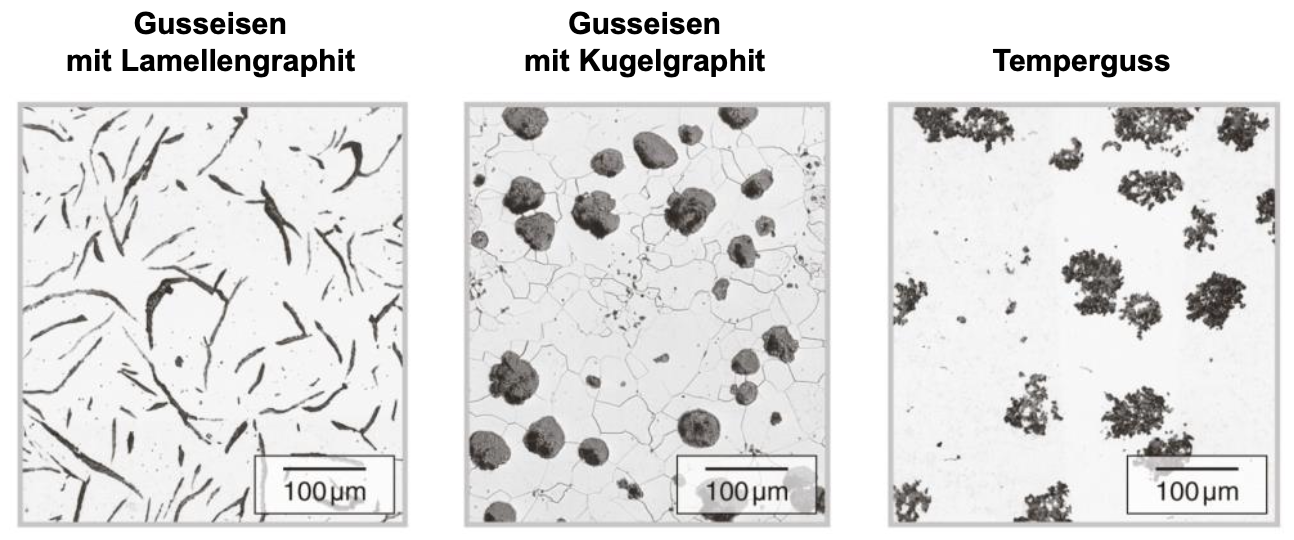
\includegraphics[width =\linewidth]{src/images/Gusseisen.png}\\

\textbf{Lamellengraphit:} gute Dämpfungs- und Wärmeleitfähigkeit, spröde 
und anfällig für Rissbildung\\

\textbf{Kugelgraphit:} hohe Festigkeit, Bruchdehnung und gute Duktilität\\

\textbf{Temperguss:} gute Duktilität und Verformbarkeit (dynamisch beanspruchte Bauteile)\\

    \subsection*{Erstarrung}
    \begin{tiny}
\begin{minipage}{0.5\linewidth}
    \[
    \boxed{        
        \begin{aligned}
            t_E &= C \cdot M^n\\
            M &= \frac{V}{A_{eff}}\\
            A_{eff} &= \varepsilon \cdot A
        \end{aligned}
    }
    \]
\end{minipage}
\begin{minipage}{0.5\linewidth}
        \item $t_E$: Erstarrungszeit
        \item $C$: Materielkonst. (Stahl 3, Eisen 5-6, Alu 6)
        \item $M$: Modul
        \item $\varepsilon $: Dehnung
\end{minipage}
\vspace{1mm}
\end{tiny}
\begin{center}
   $M_{\text{Speiser}} > M_{\text{Gussstück}}$ 
\end{center}

    \subsubsection*{Exogene Erstarrung}
    \begin{minipage}{0.6\linewidth}
    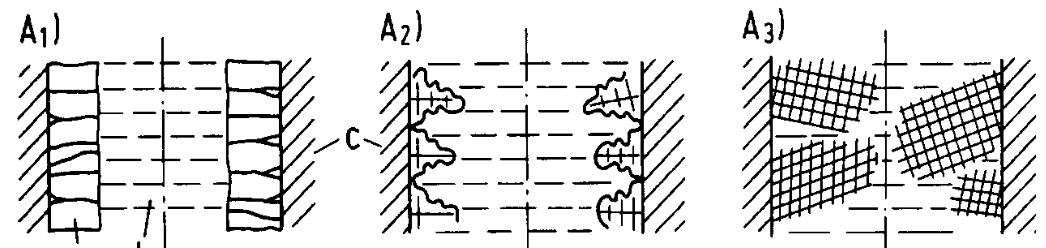
\includegraphics[width = 40mm]{src/images/Exogene Erstarrung.png}
\end{minipage}
\begin{minipage}{0.3\linewidth}
    A1: glattwandig\\
    A2: rauwandig\\
    A3: schwammartig
\end{minipage}

    \subsubsection*{Endogene Erstarrung}
    \begin{minipage}{0.6\linewidth}
    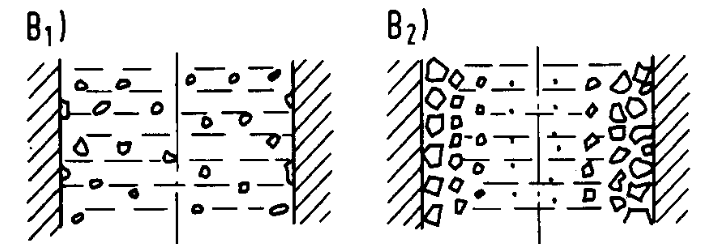
\includegraphics[width = 40mm]{src/images/Endogene Erstarrung.png}
\end{minipage}
\begin{minipage}{0.3\linewidth}
    B1: breiartig\\
    B2: schalenbildend\\
\end{minipage}
    \subsubsection*{Erstarrungsmodelle}
    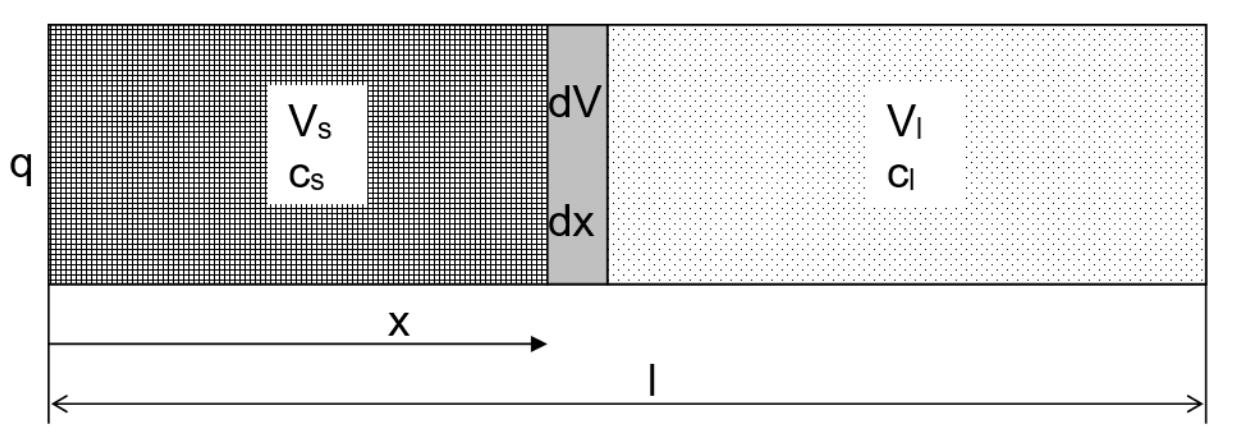
\includegraphics[width = 70mm]{src/images/Tiegel.png}
Vollst. Konzentrationsausgl. im Festen und in der Schmelze:

\[
\boxed{
    \begin{aligned}
        c_s = k \cdot c_l \Leftrightarrow c_s = k \cdot c_0 \cdot \frac{l}{l - x \cdot(1 - k)}
    \end{aligned}
}
\]
    \subsubsection*{Diffusion}
    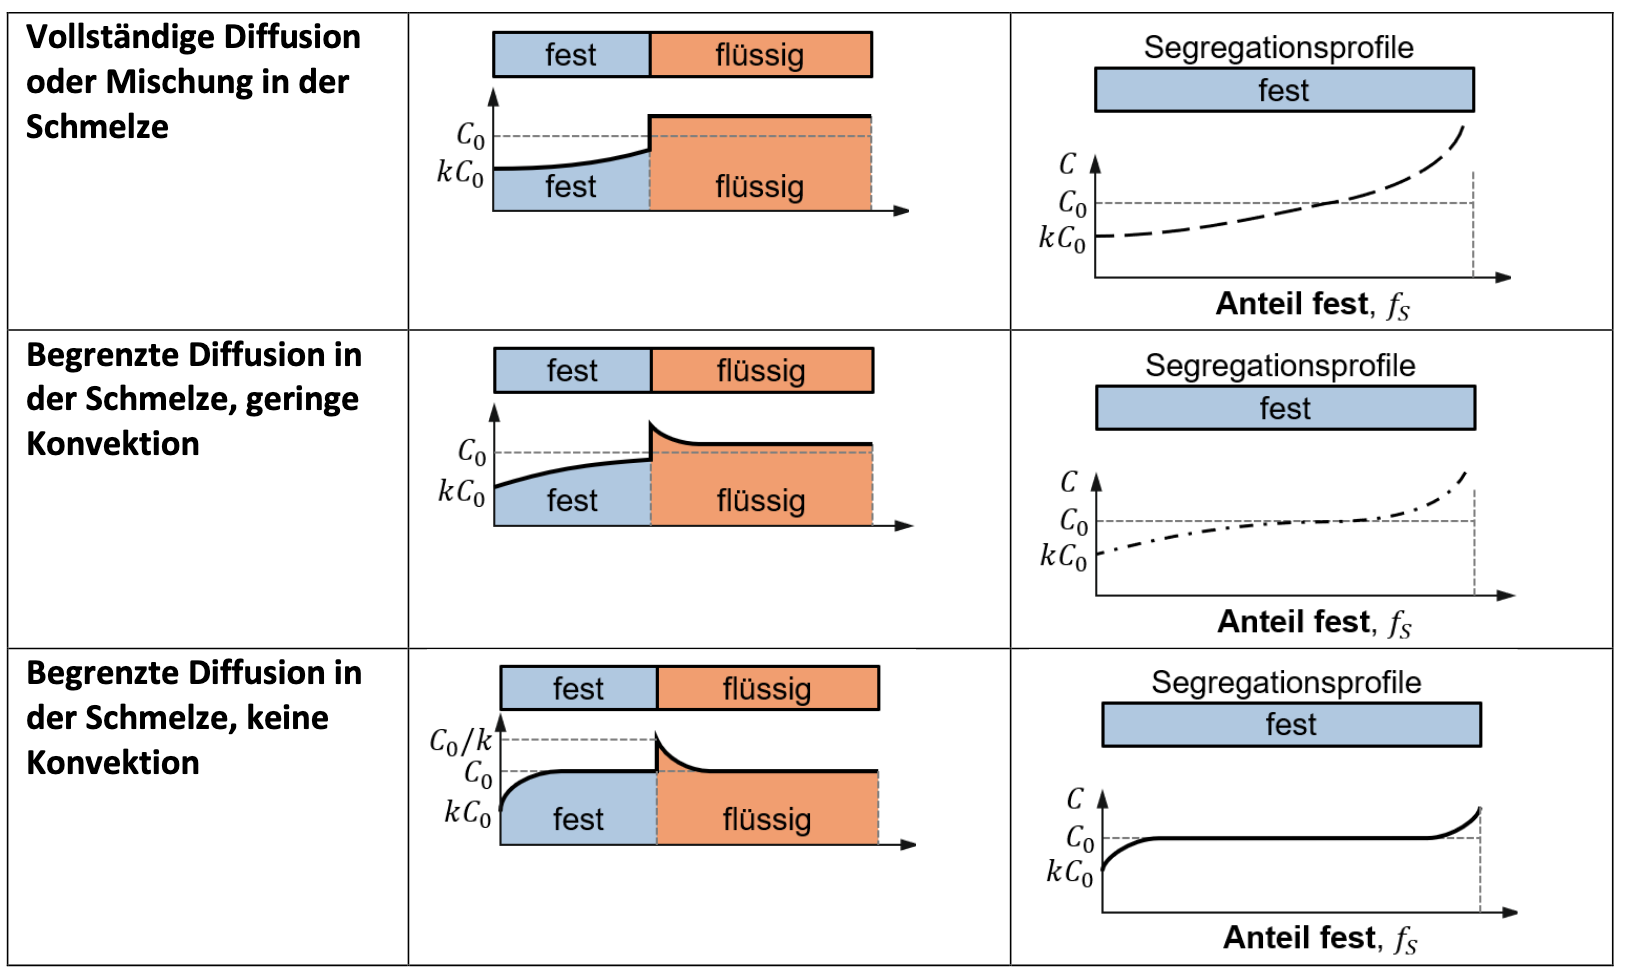
\includegraphics[width = 70mm]{src/images/Diffusion1.png}

\begin{center}
    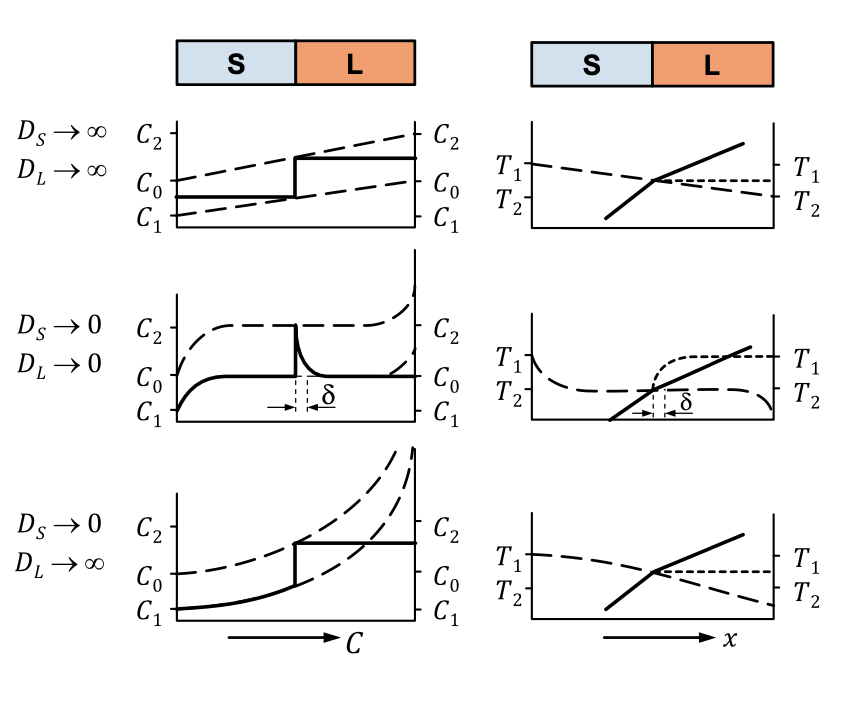
\includegraphics[width = 50mm]{src/images/Diffusion2.png}
\end{center}


    \subsection*{Keimbildung}
    \begin{minipage}{0.5\linewidth}
    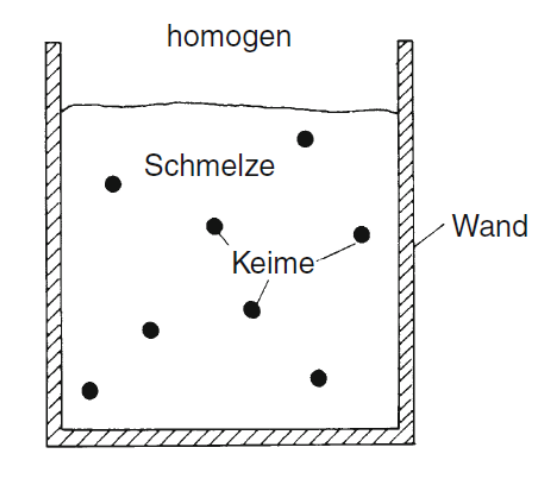
\includegraphics[width = 35mm]{src/images/Homogen.png}
\end{minipage}
\begin{minipage}{0.5\linewidth}
    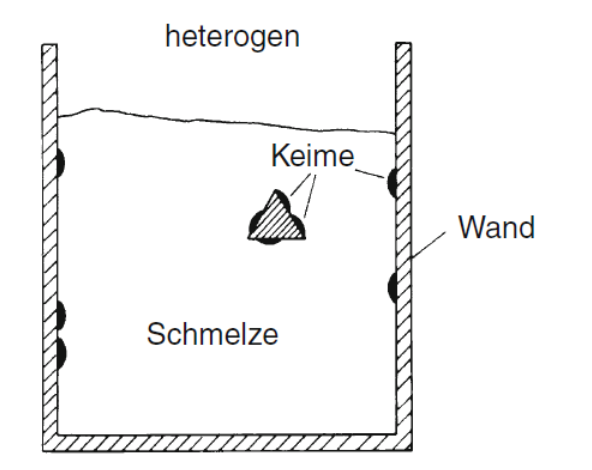
\includegraphics[width = 35mm]{src/images/Heterogen.png}
\end{minipage}
\item Homogen: einheitliches Gemisch (gleiche Phase), 
nur bei starker Unterkühlung
\item Heterogen: Keime bilden sich um Verunreinigungen\\
    \subsubsection*{Thermodynamik}
    \begin{tiny}
\begin{minipage}{0.5\linewidth}
    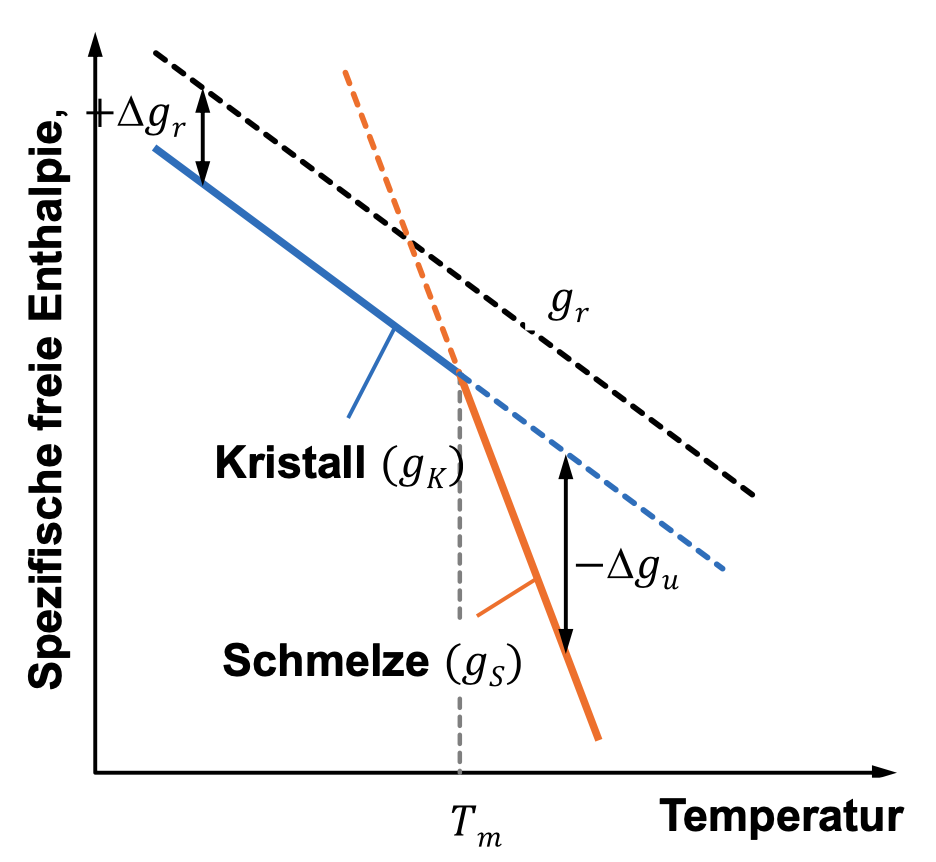
\includegraphics[width = 35mm]{src/images/Thermo_Erstarrung.png}

\end{minipage}
\begin{minipage}{0.5\linewidth}
    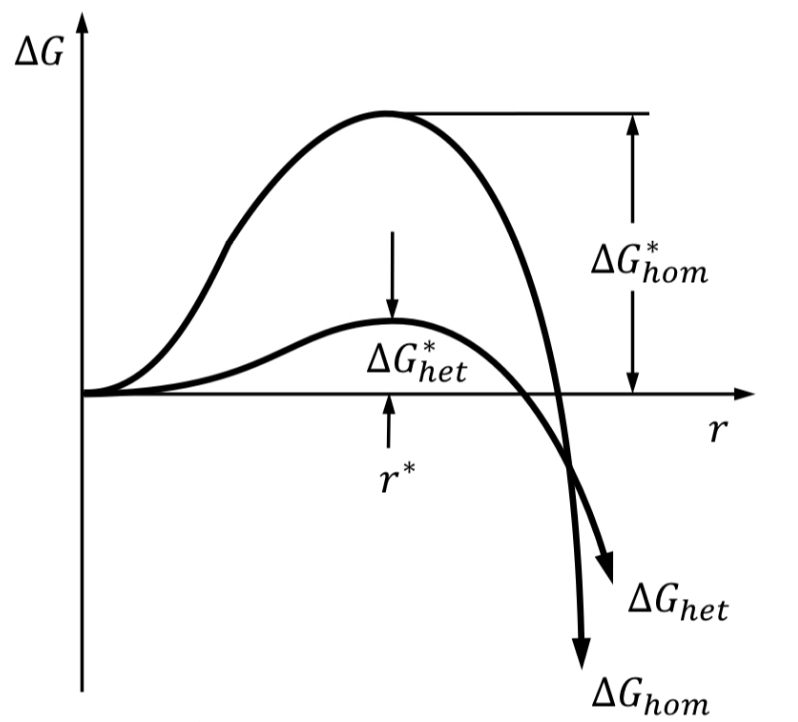
\includegraphics[width = 35mm]{src/images/Embryo_vs_Keim.png}

\end{minipage}

\begin{minipage}{0.5\linewidth}
    Unterkühlung: 
    $ \Delta g_u = g_s - g_K$\\
\end{minipage}
\begin{minipage}{0.5\linewidth}

    
    \begin{center}
        \begin{align*}
            \Delta G_u(r) &= - \frac{4}{3}\pi r^3\Delta g_u\\
            \Delta G_G(r) &= 4\pi r^2 \sigma
        \end{align*}
    \end{center}
\end{minipage}
\vspace{2mm}


\begin{minipage}{0.55\linewidth}
    Ein Keim kann nur dann wachsen wenn die \\
    freiwerdendende Umwandlungsenergie $\Delta G_u(r)$ grösser ist als die Grenzflächenenergie $\Delta G_G(r)$
\end{minipage}
\begin{minipage}{0.45\linewidth}
    \begin{center}
        $\left| \frac{d \Delta G_u(r)}{dr} \right| > \left| \frac{d \Delta G_G(r)}{dr} \right|$\\  
    \end{center}
\end{minipage}
\vspace{1mm}
\end{tiny}

\begin{minipage}{0.6\linewidth}
    \textbf{Kritischer Radius:} Min. Radius damit Keim wächst
\end{minipage}
\begin{minipage}{0.4\linewidth}
    \[
        \boxed{       
            \begin{aligned}
                r^{*} &= \frac{2\sigma}{\Delta g_u}
            \end{aligned}
        }
    \]
\end{minipage}

\vspace{1mm}

\begin{minipage}{0.6\linewidth}
    \textbf{Dentritenarmabstand:}
\end{minipage}
\begin{minipage}{0.4\linewidth}
    \[
        \boxed{       
            \begin{aligned}
                DAS &= A \cdot t^{\frac{1}{3}}_{E}
            \end{aligned}
        }
    \]
\end{minipage}
\vspace{1mm}

Falls Abkühlrate $\uparrow $ :  lokale Erstarrungszeit $\downarrow $ und DAS $\downarrow $\\



    \subsection*{Mechanischen Eigenschaften und Abkühlrate}
    \input{src/5_Urformen/Mechanischen Eigenschaften und Abkühlrate.tex}
    \subsection*{Auslegung Giessprozess}
    \begin{minipage}{0.6\linewidth}
    \textbf{Formfüllungsvermögen:}
\end{minipage}
\begin{minipage}{0.4\linewidth}
    \[
        \boxed{       
            \begin{aligned}
                F=\frac{\rho \cdot g \cdot h}{2\cdot \sigma} \\
            \end{aligned}
        }
    \]
\end{minipage}
\vspace{1mm}

\begin{minipage}{0.6\linewidth}
    \textbf{Strömungsgeschwindigkeit:}
\end{minipage}
\begin{minipage}{0.4\linewidth}
    \[
        \boxed{       
            \begin{aligned}
                v_1=\frac{\pi \cdot D^2}{4 \cdot A_1}\cdot v_K\\            
            \end{aligned}
        }
    \]
\end{minipage}
\vspace{1mm}

\begin{minipage}{0.6\linewidth}
    \textbf{Giessleitung und Querschnitt:}
\end{minipage}
\begin{minipage}{0.4\linewidth}
    \[
        \boxed{       
            \begin{aligned}
                A=\frac{Q}{\sqrt{2\cdot g \cdot h}}\\           
            \end{aligned}
        }
    \]
\end{minipage}
\vspace{1mm}
    \subsection*{Eisenkohlenstoffdiagramm $\heartsuit$}
    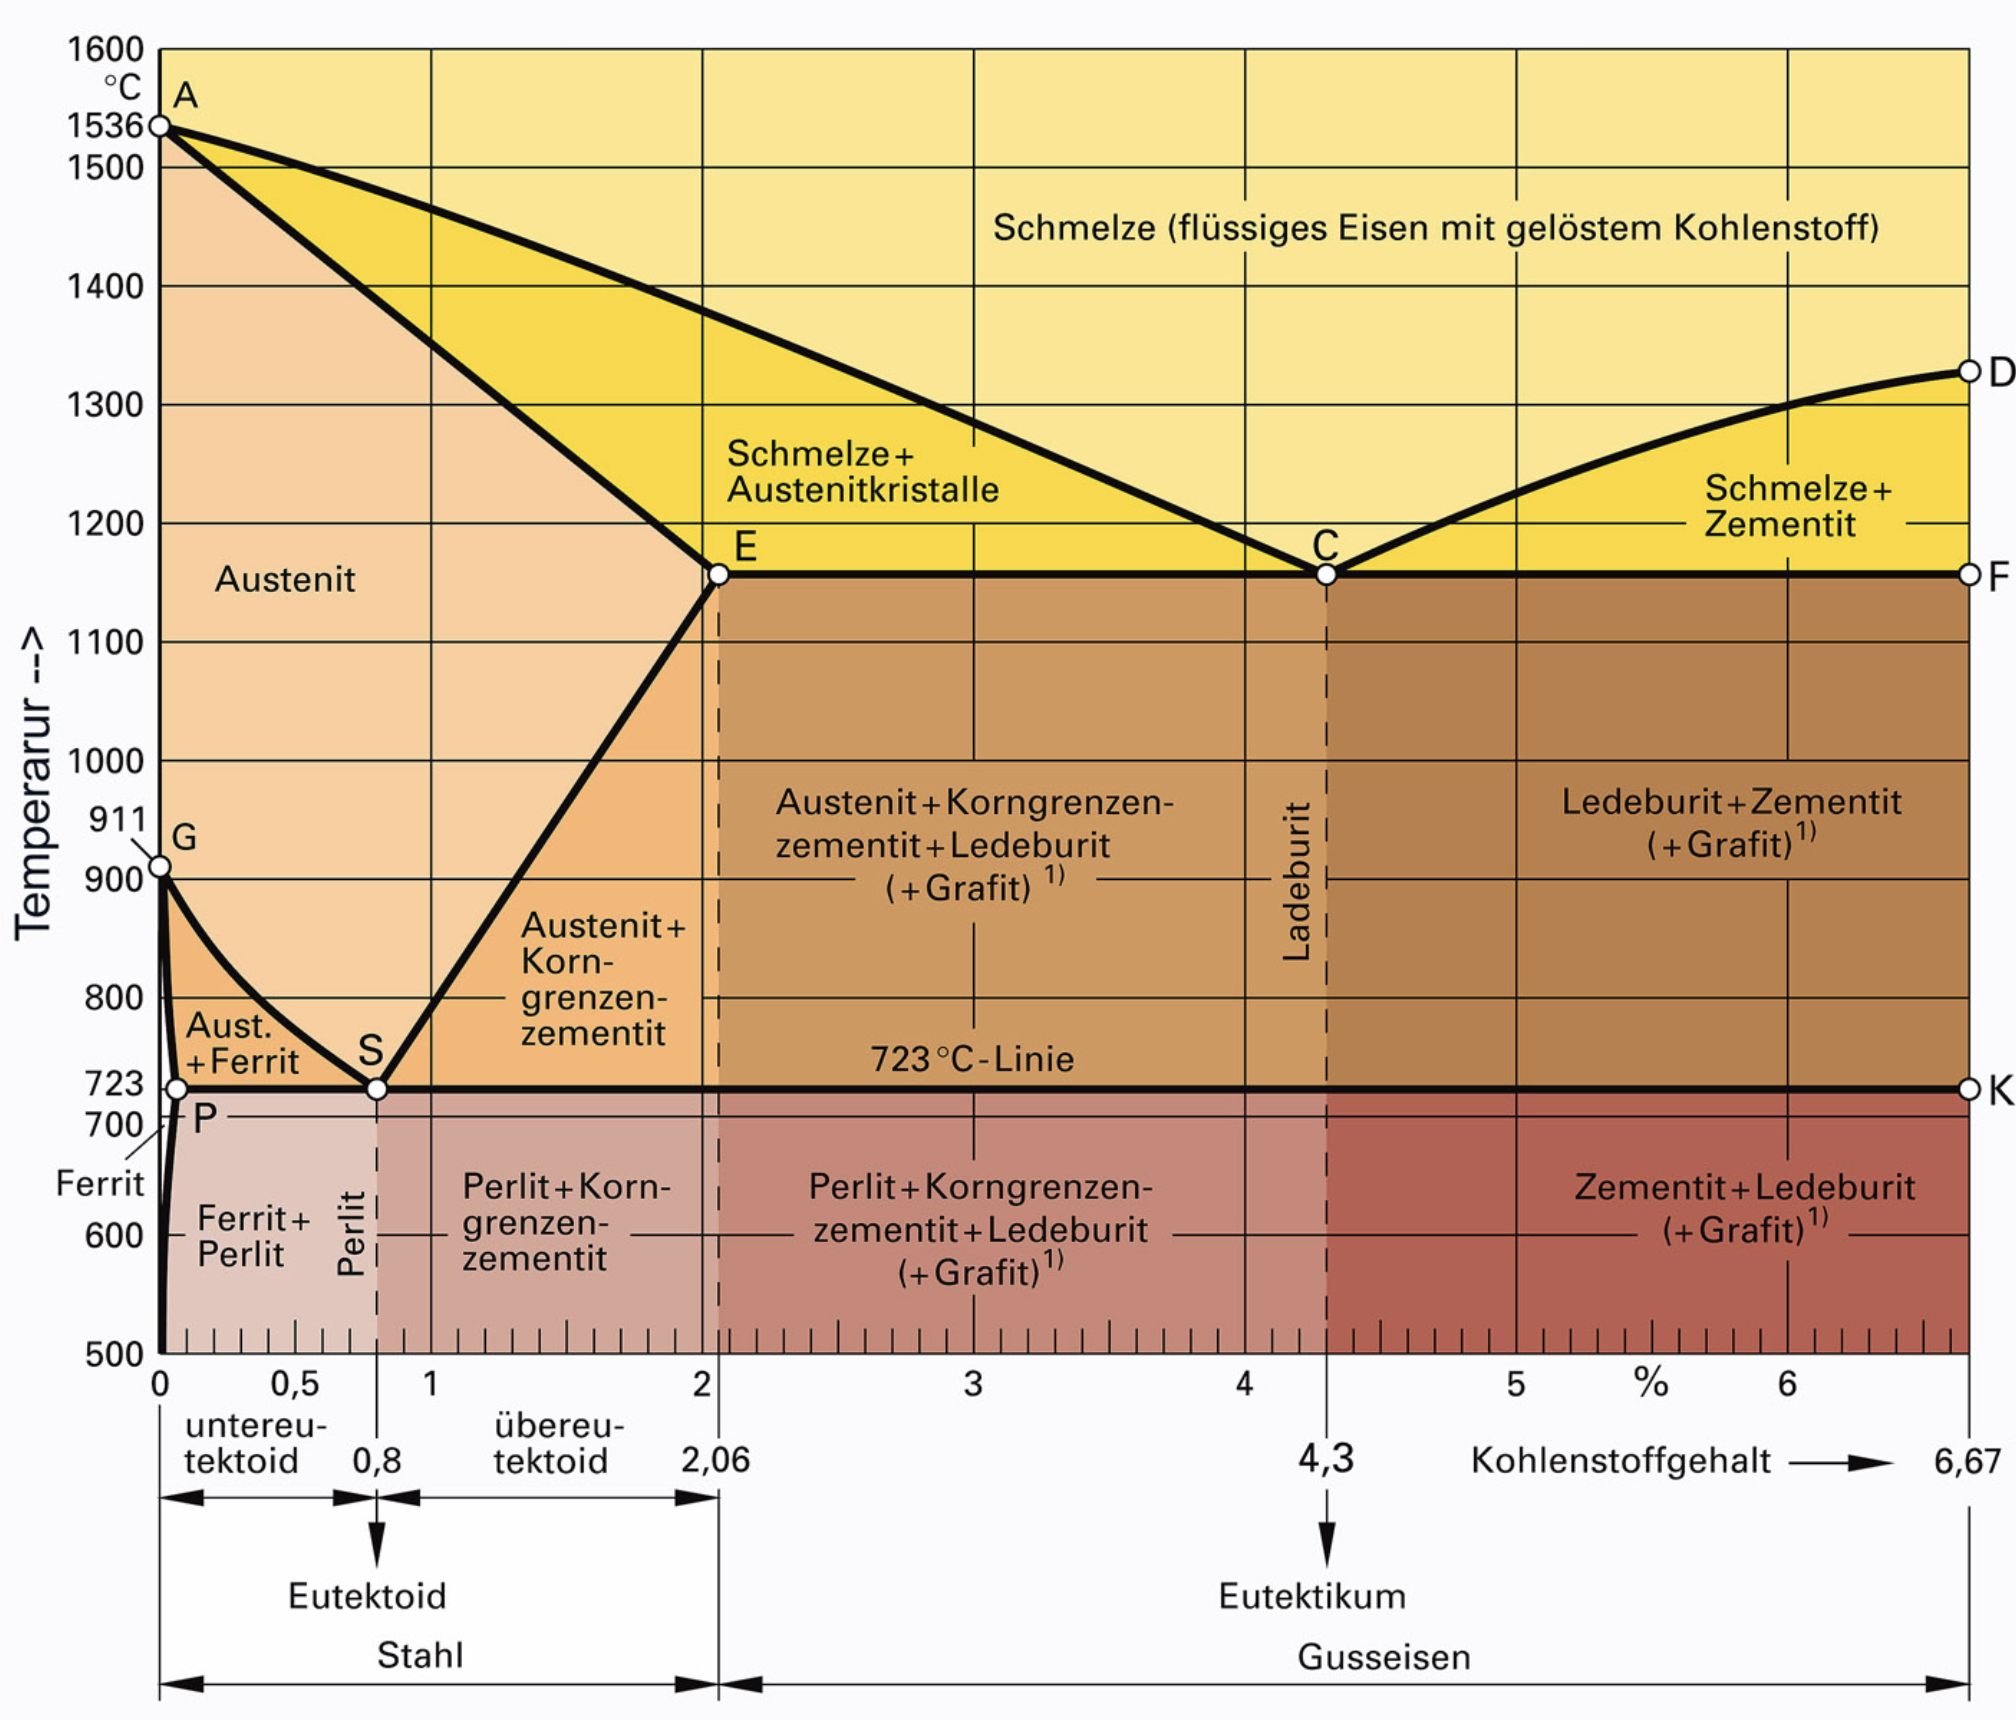
\includegraphics[width = 70mm]{src/images/Eisenkohlenstoffdiagramm.png}
\begin{minipage}{0.39\linewidth}
    \begin{itemize}
        \item Austenit = $\gamma$\\
        \item Ferrit = $\alpha$\\
        \item Zementit = $Fe_3C$\\
    \end{itemize}
\end{minipage}
\begin{minipage}{0.62\linewidth}
    \begin{itemize}
        \item Perlit = Ferrit + Zementit\\
        \item Ledeburit I = Austenit + Zementit\\
        \item Ledeburit II = Perlit + Zementit\\    
    \end{itemize}
\end{minipage}

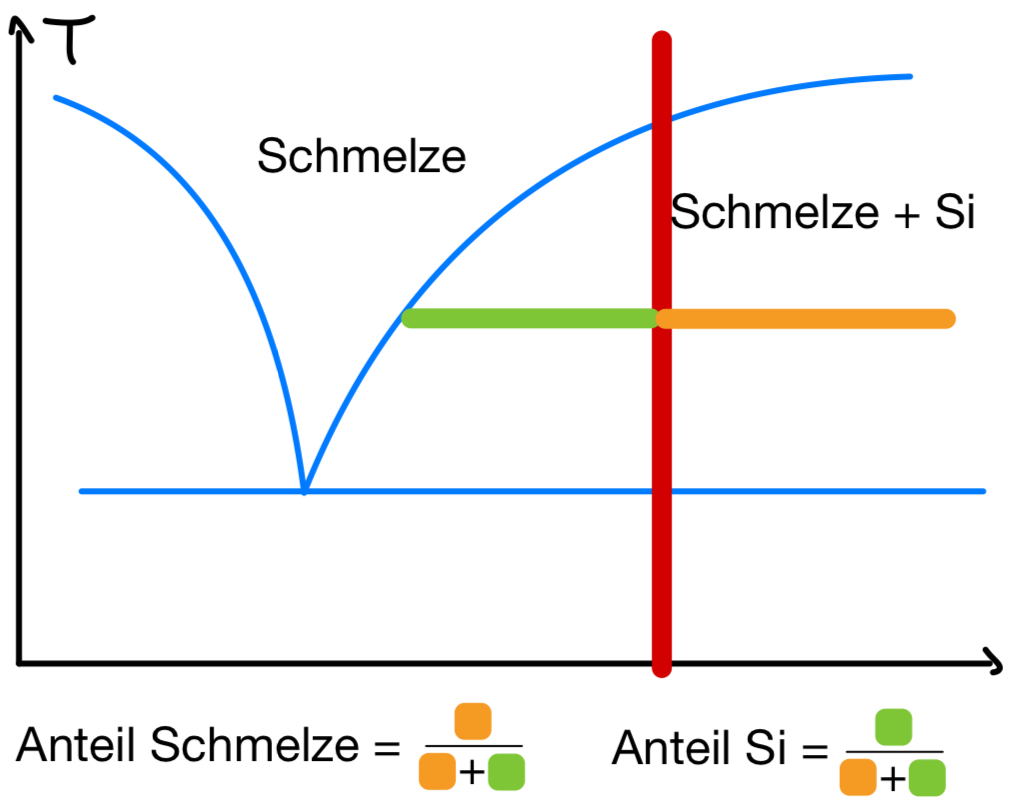
\includegraphics[width = 70mm]{src/images/Hebelgesetz.jpeg}

\begin{minipage}{0.6\linewidth}
    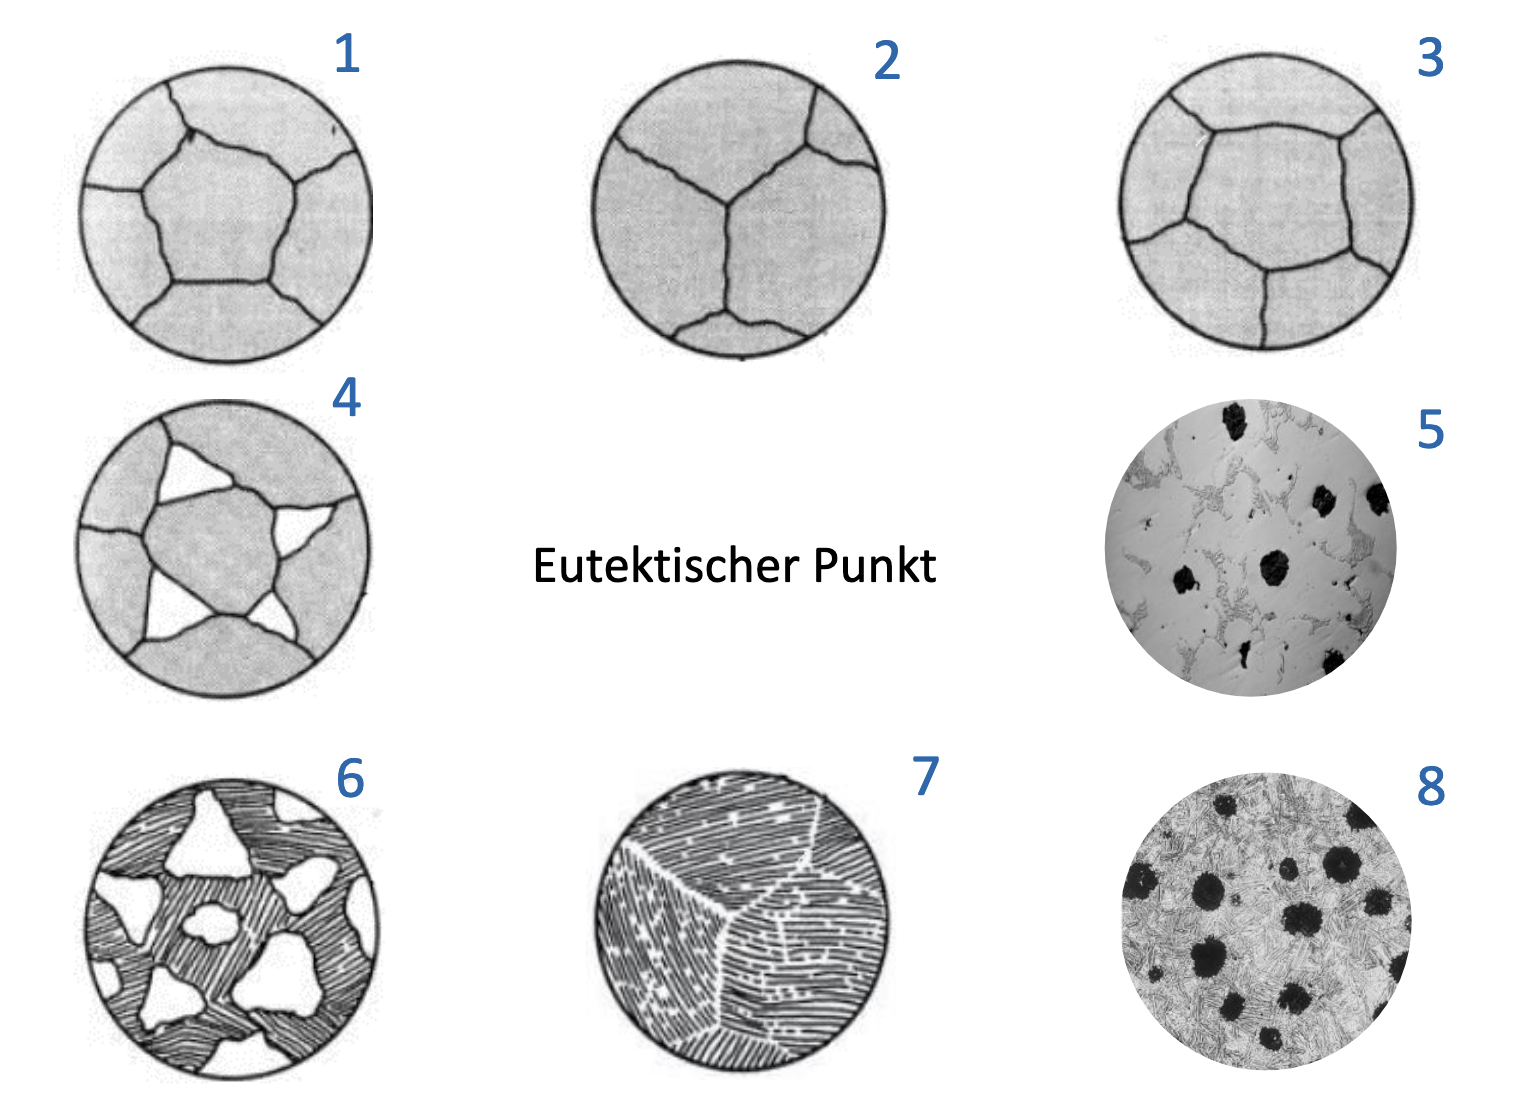
\includegraphics[width = 40mm]{src/images/Kreisli.png}
\end{minipage}
\begin{minipage}{0.4\linewidth}
    1 - 3: Austenit\\
    4: Austenit + Ferrit\\
    5: Austenit + Graphit\\
    6: Perlit + Ferrit\\
    7: Perlit\\
    8: Perlit + Graphit\\
\end{minipage}


    \vfill \null \columnbreak


\section*{Pulvermetallurgie}
    \textbf{Eigenschaften:}
\begin{itemize}
    \item komplexe Formen mit engen Toleranzen
    \item nicht Energieaufwendig
    \item Mechanische Eigenschaften einstellbar
    \item Hohe Rohstoffausnutzung
    \item $\uparrow$ Porosität, $\downarrow$ Bruchdehnung, $\downarrow$ Festigkeit
\end{itemize}

    \subsection*{Pulverherstellung}
    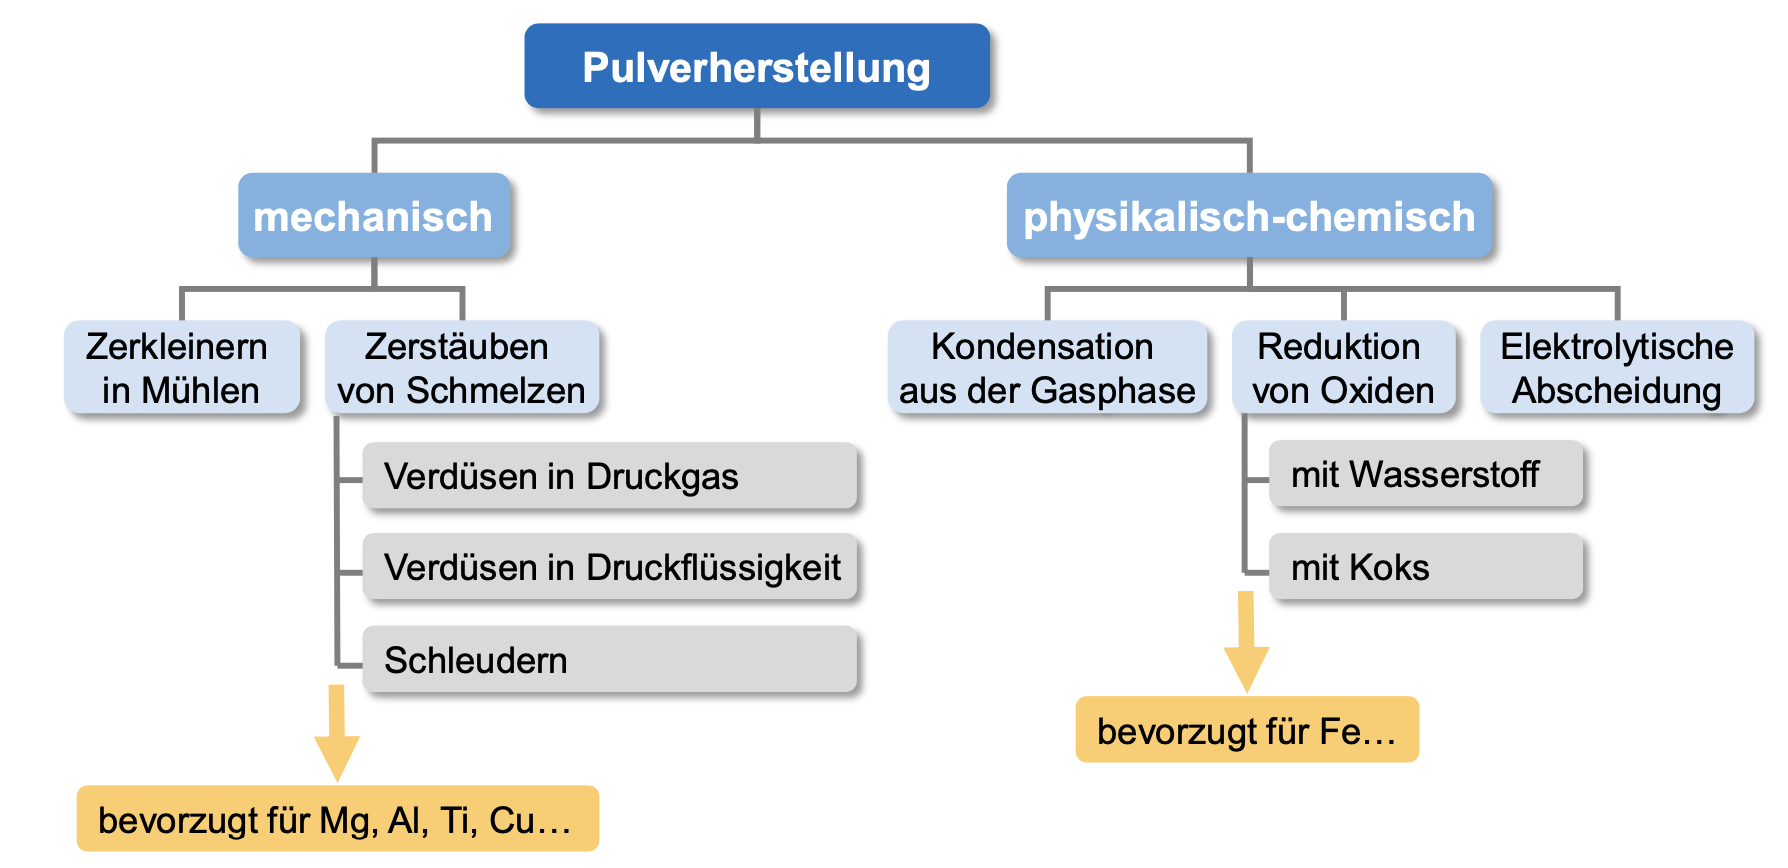
\includegraphics[width = 70mm]{src/images/Pulverherstellung.png}

\includegraphics[width = 70mm]{src/images/Verdüsen.png}
\begin{minipage}{0.5\linewidth}
    Verdüsen im Druckgas
    \begin{tiny}
        \begin{itemize}
            \item Kugelförmig
            \item 1 - 150 $\mu m$
        \end{itemize}
    \end{tiny}
\end{minipage}
\begin{minipage}{0.5\linewidth}
    Verdüsen in Druckflüssigkeit
    \begin{tiny}
        \begin{itemize}
            \item Unregelmäßig
            \item 50 - 500 $\mu m$
            \item Kostengünstig
        \end{itemize}
    \end{tiny}
\end{minipage}

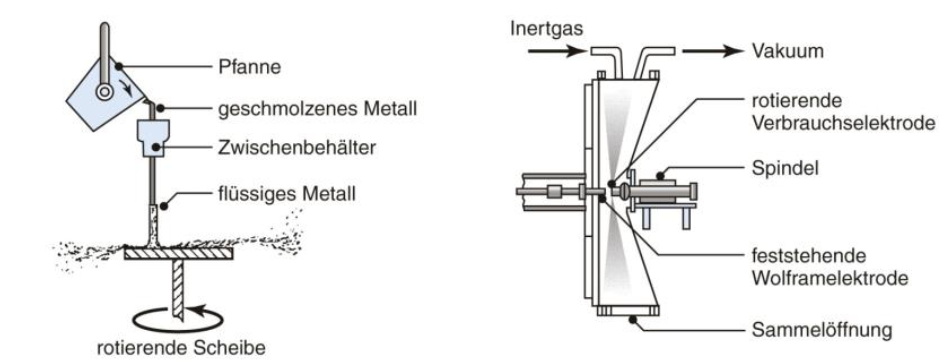
\includegraphics[width = 70mm]{src/images/Schleudern:Elektrolytisch.png}
\begin{minipage}{0.5\linewidth}
    Schleudern
    \begin{tiny}
        \begin{itemize}
            \item Kugelförmig
            \item 50 - 500 $\mu m$
            \item Kühlt Legierung schnell Abkühlrate
            \item Hohe Reinheit
        \end{itemize}
    \end{tiny}
\end{minipage}
\begin{minipage}{0.5\linewidth}
    Elektrolytische Abscheidung
    \begin{tiny}
        \begin{itemize}
            \item Kugelförmig
            \item 10 - 100 $\mu m$
            \item extrem fein
            \item Reines und gleichmässigs Pulver
        \end{itemize}
    \end{tiny}
\end{minipage}




    \subsection*{Kennwerte}
    \begin{tiny}
    \begin{align*}
    d_{50} &= \text{Medianwert, 50\% der Partikel sind kleiner als dieser Wert} \\
    d_{90} &= \text{90\% der Partikel sind kleiner als dieser Wert} \\
    d_{10} &= \text{10\% der Partikel sind kleiner als dieser Wert} \\
    | d_{90} - d_{10} | &= \text{Spannweite}
\end{align*}
\end{tiny}


\textbf{Mastersinterkurve:}
rel. Dichte $\rho (t,T)$  vs log. Sinterarbeit $\log \Theta $\\
Unabhängig der Heizrate folgen alle Kurven dem gleichen Trend\\

\textbf{Annahmen}: Es existiert nur ein einzelner Diffusionsmechanismus, 
Diffusion thermisch aktiviert, Korngröße/Mikrostruktur variiert 
nur mit der Dichte, Oberflächendiffusion vernachlässigt.\\

\textbf{Einschränkungen}: $Q$ (Aufheizrate) hängt von der Partikelgrössen-\\
verteilung (PSD) und der Chemie ab. MSC ist empfindlich für 
Änderungen in der Materialzusammensetzung und Prozessbedingungen.\\
Bei $\rho (t,T) > 90 \%$ nimmt $Q$ ab.\\
    \vfill \null \columnbreak
    \subsection*{Sintern}
    \textbf{Grünkörper} (fein/grobkörniges Metall/Keramikpulver) wird durch 
Wärmebehandlung zu einem festen Werkstück gesintert.\\
Gesinterte Teile sind deshalb nicht homogen (im Gegensatz zu 
Metalllegierungen) und können eine \textbf{Porosität} aufweisen. Diese lässt 
sich durch Kompaktieren modifizieren.\\
Durch Sintern lassen sich Stoffe zusammenbringen die auf andere 
Weise schwer oder nicht vereinbar sind.\\
Die Pulverzusammensetzung kann während des Sinterns verändert werden.\\

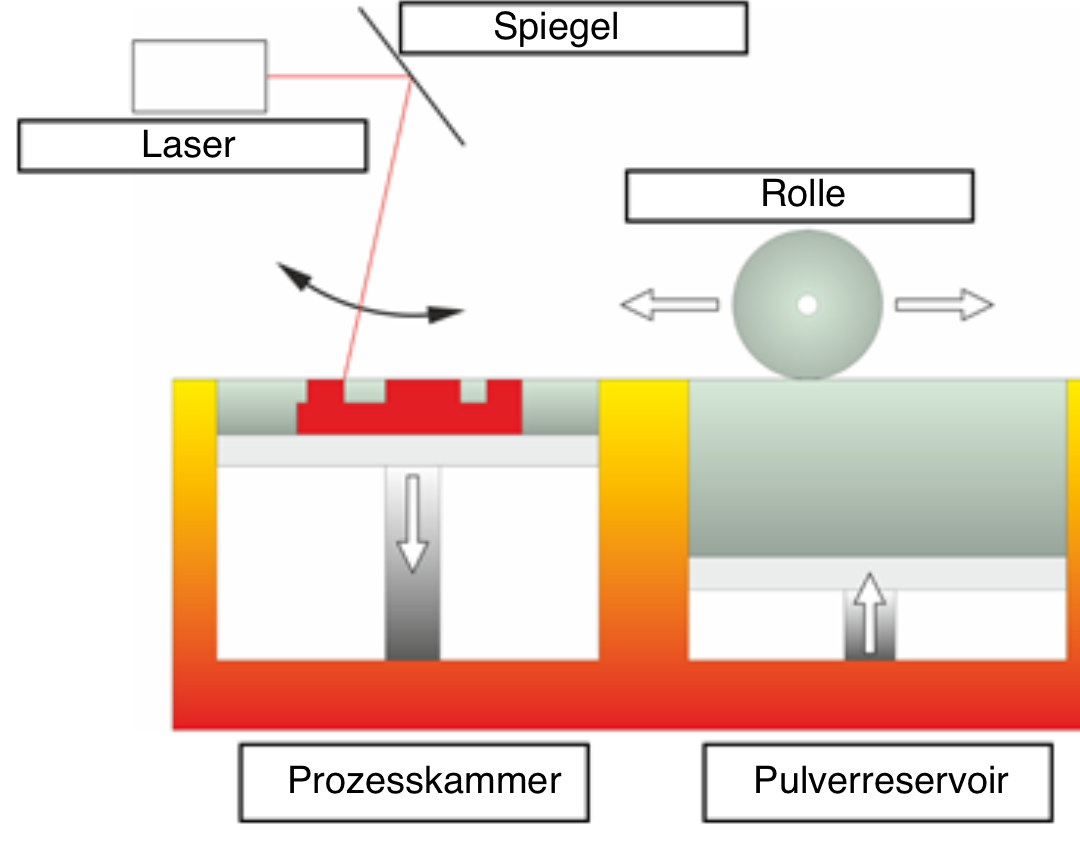
\includegraphics[width =0.6\linewidth]{src/images/Sintern.png}\\

    \subsection*{Formeln zur Pulvermetallurgie}
    \textbf{Ball Milling:}\\

\begin{minipage}{0.5\linewidth}
    \[
    \boxed{        
            \omega_{K} = \frac{42.2}{D - d}
    }
    \]
\end{minipage}
\begin{minipage}{0.5\linewidth}
    \item $\omega_{K}$: Kritische Rotationsgeschw.
    \item $D$: Behälterdurchmesser
    \item $d$: Kugeldurchmesser
    \item Richtwert: $\omega_{K} \approx 75 \%$
\end{minipage}
\vspace{1mm}

\textbf{E-Modul als Funktion der Prorsität:}\\

\begin{minipage}{0.5\linewidth}
    \[
    \boxed{        
        E(p) = E_0 \left( 1 - \frac{p}{p_c} \right)^f    }
    \]
\end{minipage}
\begin{minipage}{0.5\linewidth}
    \item $E$: Eff. E-Modul des porösen Materials
    \item $E_0$: E-Modul des Vollmaterials
    \item $p$: Porosität
    \item $p_c$: Porosität wo $E$ verschwindet
    \item $f$: Parameter (Morphologieabhängig)
\end{minipage}
\vspace{1mm}

\textbf{Streckenenergiedichte beim sel. Laserschmelzen:}\\

\begin{minipage}{0.5\linewidth}
    \[
    \boxed{
        E_S = \frac{\textcolor{red}{P_L}}{\textcolor{green}{v_s}}
    }
    \]
\end{minipage}
\begin{minipage}{0.5\linewidth}
    \item $E_S$: Streckenenergiedichte
    \item \textcolor{red}{$P_L$}: Leistung des Lasers
    \item \textcolor{green}{$v_s$}: Belichtungsgeschwindigkeit
\end{minipage}
\vspace{1mm}

\textbf{Flächenenergiedichte beim sel. Laserschmelzen:}\\

\begin{minipage}{0.5\linewidth}
    \[
    \boxed{        
        E_A = \frac{\textcolor{red}{P_L}}{\textcolor{green}{v_s} \cdot \textcolor{blue}{h_s}}
    }
    \]
\end{minipage}
\begin{minipage}{0.5\linewidth}
    \item $E_A$: Flächenenergiedichte
    \item \textcolor{blue}{$h_s$}: Linienabstand
\end{minipage}
\vspace{1mm}

\textbf{Volumenenergiedichte beim sel. Laserschmelzen:}\\

\begin{minipage}{0.5\linewidth}
    \[
    \boxed{        
        E_V = \frac{\textcolor{red}{P_L}}{\textcolor{green}{v_s} \cdot \textcolor{blue}{h_s} \cdot s}
    }
    \]
\end{minipage}
\begin{minipage}{0.5\linewidth}
    \item $E_V$: Volumenenergiedichte
    \item $s$: Schichtdicke
\end{minipage}
\vspace{1mm}

\textbf{Gesamtenergie des Systems}\\

\begin{minipage}{0.5\linewidth}
    \[
    \boxed{        
        E_{tot} = \textcolor{orange}{\gamma _S} A_s + \textcolor{magenta}{\gamma _{GB}} A_{GB}
    }
    \]
\end{minipage}
\begin{minipage}{0.5\linewidth}
    \item \textcolor{orange}{$\gamma _S$}: Oberflächenenergie
    \item $A_s$: Oberfläche des Kristalls
    \item \textcolor{magenta}{$\gamma _{GB}$}: Energie der Korngrenze
    \item $A_{GB}$: Fläche der Korngrenze
\end{minipage}
\vspace{1mm}
\vfill \null \columnbreak

\textbf{Dihedralwinel}\\

\begin{minipage}{0.5\linewidth}
    \[
    \boxed{        
        \frac{\textcolor{magenta}{\gamma _{GB}}}{\textcolor{orange}{\gamma _S}} = 2 \cos(\frac{\phi_e}{2})
    }
    \]
\end{minipage}
\begin{minipage}{0.5\linewidth}
    \item $\phi_e$: Gleichgewichstwinkel
\end{minipage}
\vspace{1mm}

\textbf{Verdichtungsdruck}\\

\begin{minipage}{0.5\linewidth}
    \[
    \boxed{        
        p(x) = p_0 \exp \left( - \frac{4\mu x}{D} \right)
    }
    \]
\end{minipage}
\begin{minipage}{0.5\linewidth}
    \item $p_0$: Druck an Zylinderoberseite
    \item $\mu$: Reibungskoeffizient zwischen Pulver und Zylinder
    \item $x$: Abstand zur Zylinderoberseite
    \item $D$: Durchmesser des Zylinders
\end{minipage}
\vspace{1mm}
    \subsubsection*{Übung Kaltkompaktieren}
    \input{src/6_Pulvermetallurgie/Übung Kaltkompaktieren.tex}

\section*{Umformen}
    Änderung der Form, Oberfläche und Eigenschaften bei gleicher Masse und Stoffzusammenhalt.\\

\textbf{Eigenschaften:}\\
\begin{minipage}{0.5\linewidth}
    \begin{itemize}
        \item Energieeffizient
        \item Hohe Oberflächengüte
        \item grosse Kräfte nötig
        \item teure Werkzeuge
    \end{itemize}
\end{minipage}
\begin{minipage}{0.5\linewidth}
    \begin{itemize}
        \item Verschleiss und Korrosion durch Reibung
        \item Entstehung innerer Spannungen $\rightarrow$ nachfolgende Wärmebehandlung
    \end{itemize}
\end{minipage}
    \vfill \null \columnbreak
    \subsection*{Tiefziehen}
    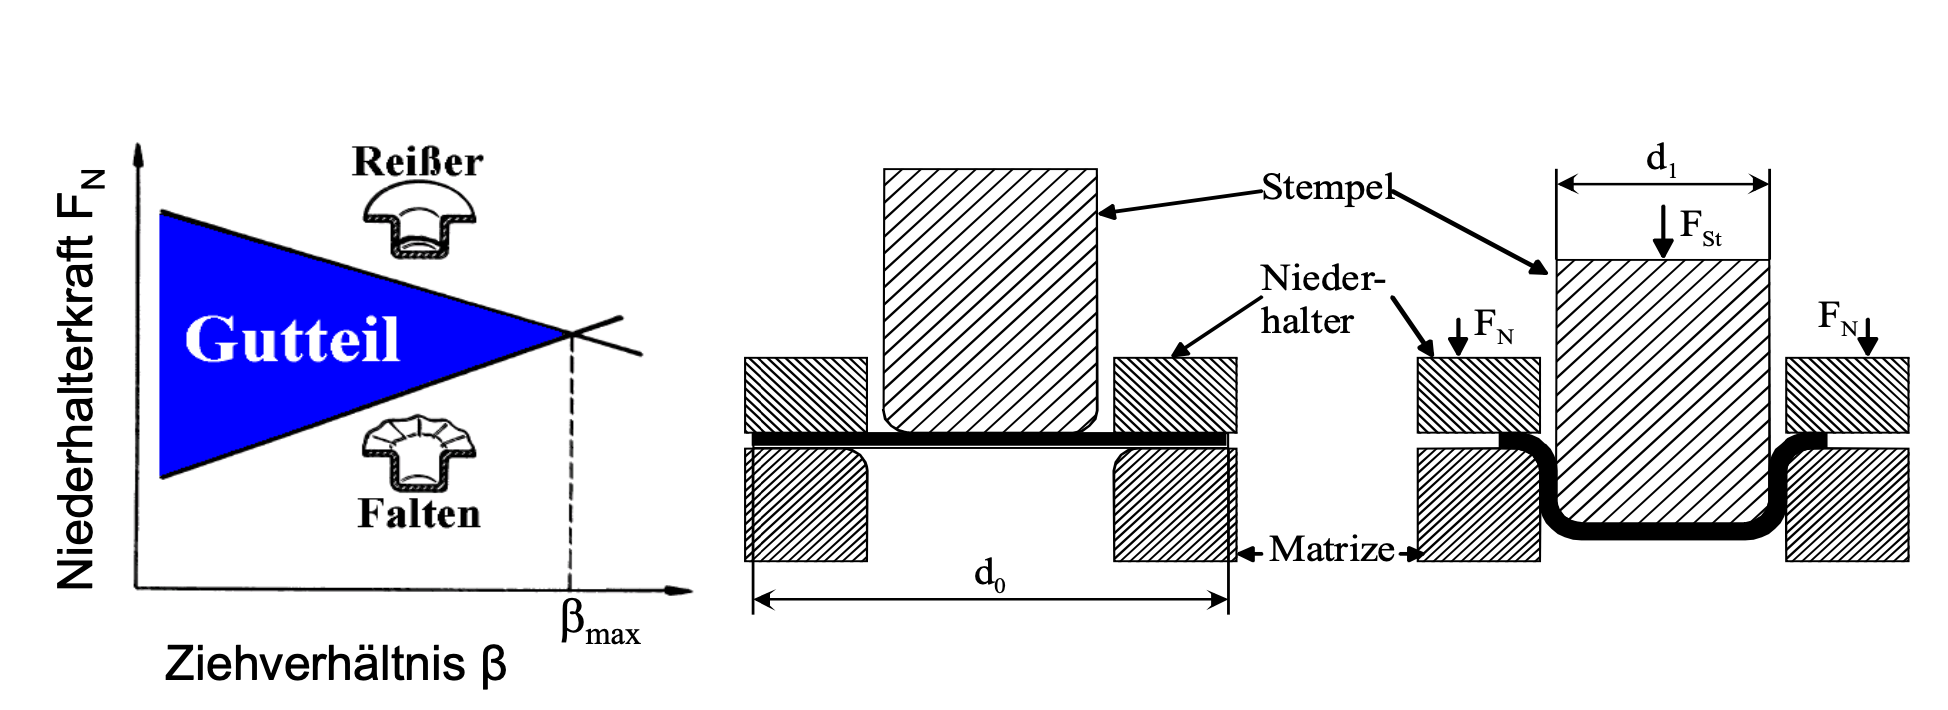
\includegraphics[width = 70mm]{src/images/Tiefziehen.png}




\begin{minipage}{0.5\linewidth}
    \[
    \boxed{     
        \begin{aligned}
            \beta &=\frac{d_0}{d_1} = \frac{d_{n - 1}}{d_n}\\
            \beta_{ges} &= \beta_1 \cdot \beta_2 ... \leq  6.5\\
            \beta_1 &\leq 2\\
            \beta_2 &\leq 1.6
        \end{aligned}
        }
    \]
\end{minipage}
\begin{minipage}{0.5\linewidth}
    \item $\beta$: Ziehverhältnis
    \item $d_0$: Durchmesser vor dem Ziehen
    \item $d_1$: Durchmesser nach dem Ziehen
    \item $\beta_{ges}$: Gesamtziehverhältnis
\end{minipage}
\vspace{1mm}

    \subsection*{Warmblechumformung/ Presshärten}
    \textbf{Vorteile:}\\
 Vermindert Rückfederung, Werkstoffe gut umformbar, Nach Härten Werkstoffe hochfest, auch für grosse Serien geeignet, Materialeigenschaften lokal einstellbar.\\

 \textbf{Verfahren:}\\
Cutting, Heating, Hot stamping, Trimming, Coating\\

\textbf{Werkzeugaufbau:}\\
\begin{minipage}{0.65\linewidth}
    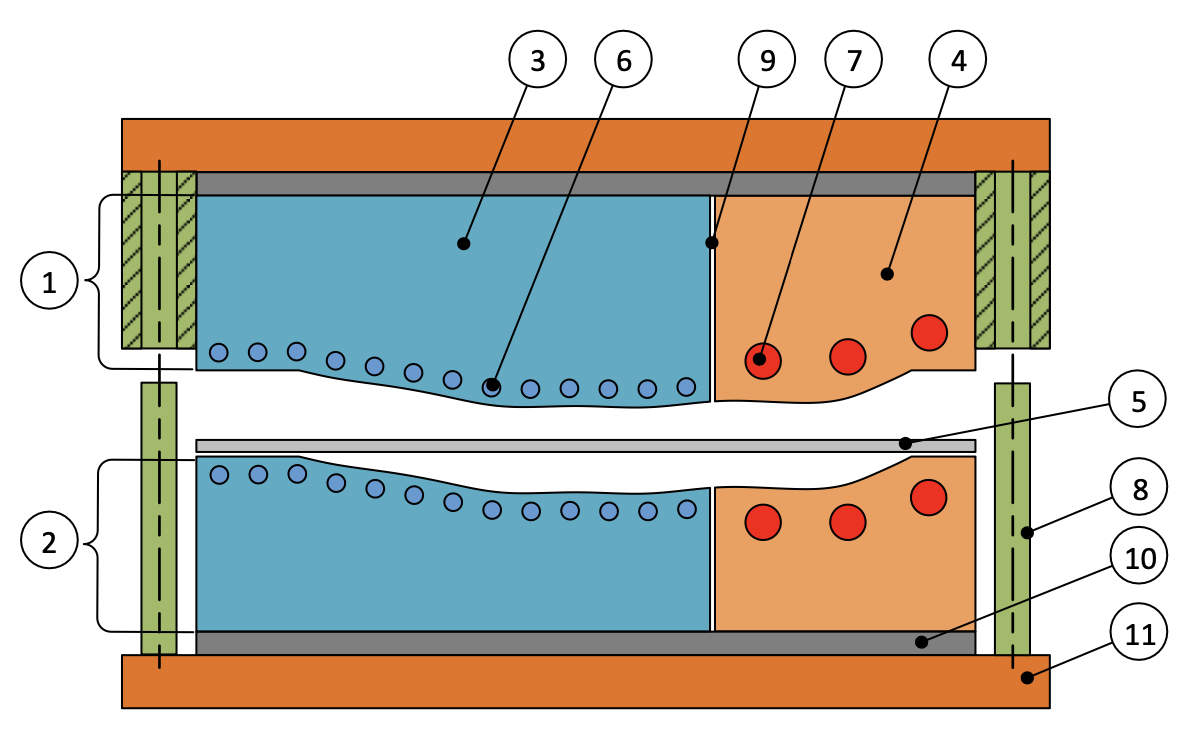
\includegraphics[width=0.8\linewidth]{src/images/Warmblechumformung.png}
\end{minipage}
\begin{minipage}{0.49\linewidth}
    \begin{tiny}
    1. Werkzeug Oberteil \\
    2. Werkzeug Unterteil \\
    3. Gekühlte Hälfte \\
    4. Temperierte Hälfte \\
    5. Blech
    6. Kühlkanal \\
    7. Heizpatrone \\
    8. Führung \\
    10. Stössel\\
    11. Grundplatte
    \end{tiny}
\end{minipage}
    \subsection*{Strecken und Biegen}
    \begin{minipage}{0.49\linewidth}
    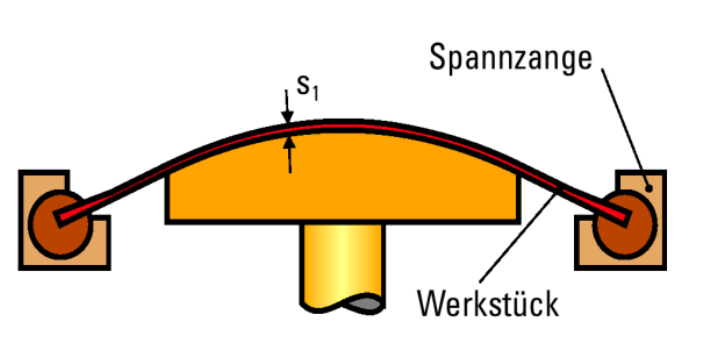
\includegraphics[width = 40mm]{src/images/Strecken.png}
\end{minipage}
\begin{minipage}{0.49\linewidth}
    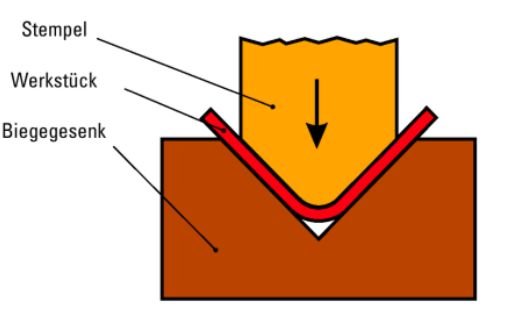
\includegraphics[width = 40mm]{src/images/Biegen.png}
\end{minipage} \\
    \subsection*{Walzen}
    \begin{center}
    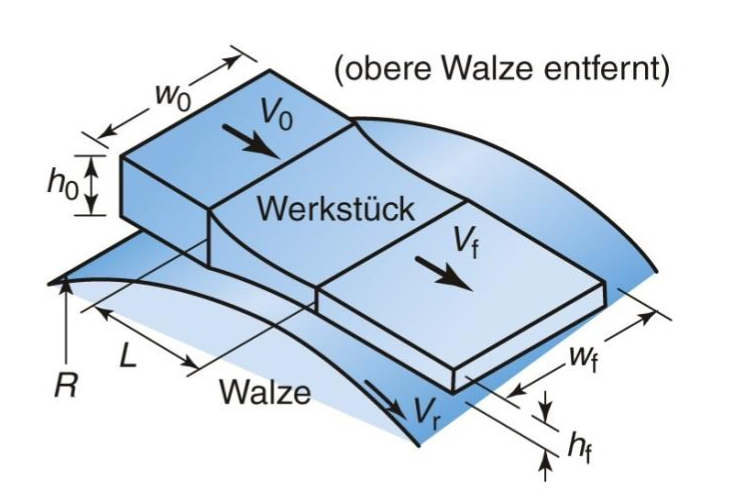
\includegraphics[width = 40mm]{src/images/Walzen.png}\\
\end{center}
\textbf{Ziel:}\\
$\downarrow$ Dicke, $\downarrow$ Fehler aus dem Giessprozess, Einstellen mechanischer Eigenschaften (Festigkeit, Textur).\\

\textbf{Warmwalzen:}\\
$\downarrow$ der Korngrösse, $\uparrow $ mechanischen Eigenschaften. \\
Warmwalzen erzeugt eine schlechtere Oberfläche als Kaltwalzen.\\
\vfill \null \columnbreak

\textbf{Durchbiegung:}\\
Führt zu Ausbauchung im Werkstoff.\\
Gegenmassnahmen: 
Stützwalzen, Vorspannung oder konvexe Walzen\\

    \subsubsection*{Walzfehler}
    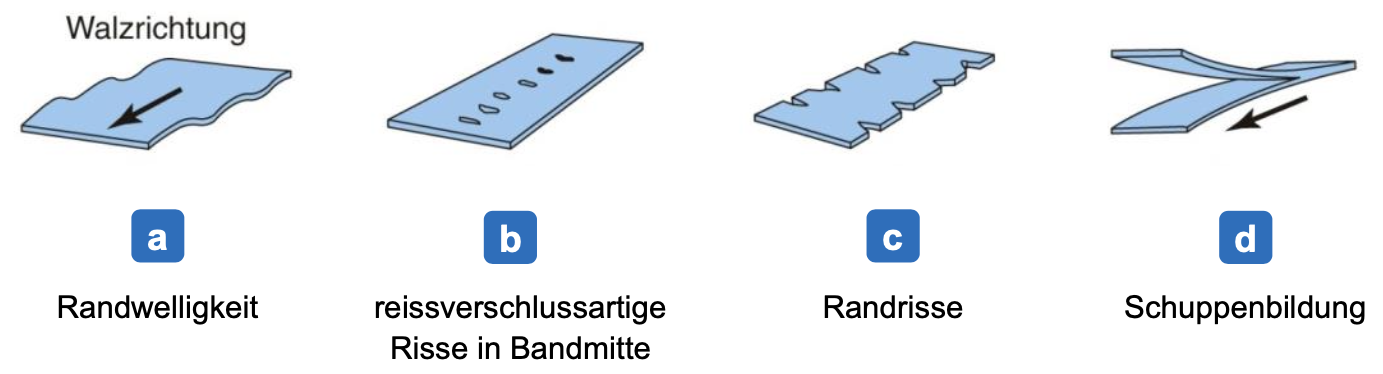
\includegraphics[width = 70mm]{src/images/Walzfehler.png}\\
    \subsection*{Gesenkschmieden}
    \begin{minipage}{0.49\linewidth}
    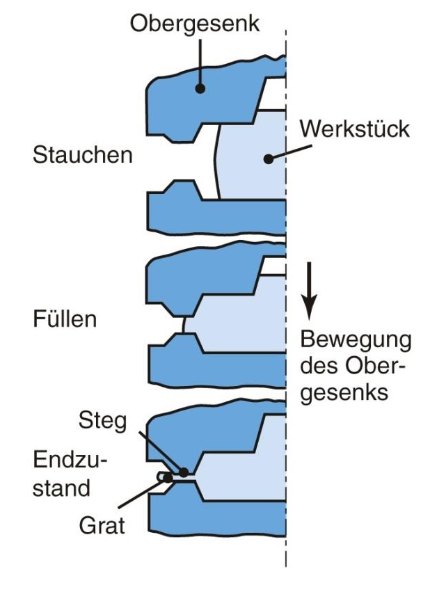
\includegraphics[width = 30mm]{src/images/Gesenkschmieden.png}
\end{minipage}
\begin{minipage}{0.49\linewidth}
    \textbf{Verfahren:}\\
    Umformen in geschlossenem Werkzeug (Gesenk).\\
    Bei sicherheitsrelevanten Teilen (Zahnräder, Pleuel, Getriebeteile). \\
    
    \textbf{Besonderheiten:}\\
    Erzeugt einen günstigen Faserverlauf (reduzierte Rissempfindlichkeit).\\
    Verschleissbelastung der Form sehr hoch.\\
    
\end{minipage}

    \subsection*{An/Isotropie}
    \begin{minipage}{0.4\linewidth}
    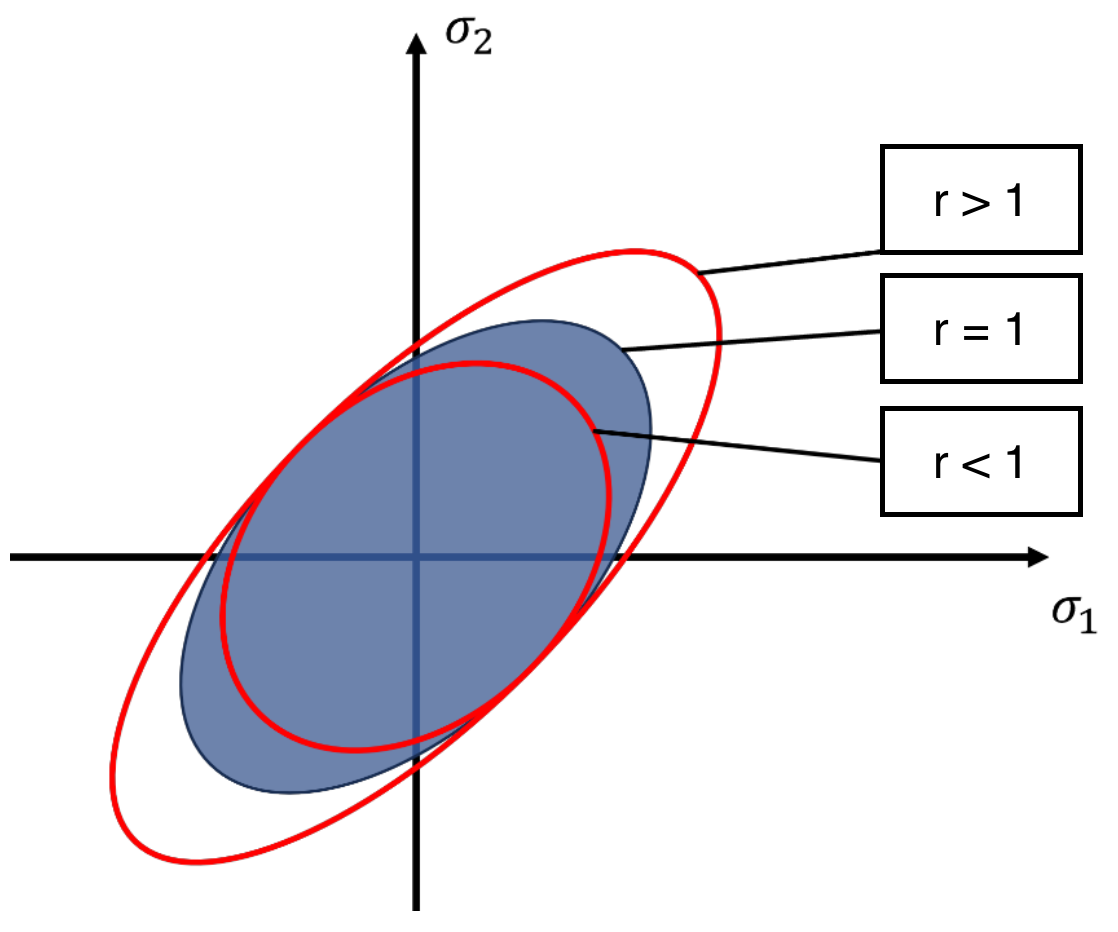
\includegraphics[width = 0.9\linewidth]{src/images/Isotropie.png}
    \mathbox{
        r = \frac{\sigma_2}{\sigma_1}
    }
\end{minipage}
\begin{minipage}{0.6\linewidth}
    \textbf{Isotropisches} Material verformt sich in 
    alle Richtungen gleich gut.\\
    r = 1\\

\textbf{Anisotropisches} Material verformt 
sich in verschiedene Richtungen unterschiedlich 
gut.\\
r $>$ 1 $\downarrow$ Dickenänderung, $\uparrow $ Breitenänderung (weniger Rissbildung)\vspace{1mm}\\
r $<$ 1 $\uparrow$ Dickenänderung, $\downarrow$ Breitenänderung
\end{minipage}
\vspace{1mm}\

Ebene Anisotropie:
Richtungsabhängigkeit der mechanischen Eigenschaften in einer Ebene.\\ 

Senkrechte Anisotropie:
Richtungsabhängigkeit der mechanischen Eigenschaften senkrecht zur Ebene.\\
    \subsection*{Formeln zur Umformung}
    \textbf{Biegelinie (einer Walze):}\\
\begin{minipage}{0.5\linewidth}
    \[
    \boxed{      
        \begin{aligned}
            \omega &= \frac{5 \cdot F \cdot b^4}{384 \cdot E \cdot I}\\
            I &= \frac{\pi  \cdot D^4}{64}
        \end{aligned}
    }
    \]
\end{minipage}
\begin{minipage}{0.5\linewidth}
    \item $\omega$: Biegelinie
    \item $F$: Streckenlast
    \item $b$: Blechbreite
    \item $I$: Flächenträgheitsmoment
    \item $D$: Walzendurchmesser
\end{minipage}
\vspace{1mm}

\textbf{Zipfelbildung:}\\
\[
\boxed{      
    \begin{aligned}
        \Delta r &= \frac{1}{2}\cdot(r_0^\circ - 2\cdot r_{45}^\circ + r_{90}^\circ)\\
        &= 2\cdot(\bar{r} - r_{45}^\circ)
    \end{aligned}
}
\]

$\Delta r > 0$: Zipfel in $0^\circ$ und $90^\circ$-Richtung\\
$\Delta r < 0$: Zipfel in den beiden Diagonalrichtungen\\
\vfill \null \columnbreak


\textbf{Wahre Dehnung/Spannung/Querschnitt:}\\
\begin{minipage}{0.5\linewidth}
    \[
    \boxed{
        \begin{aligned}
            \sigma_{w} &= \sigma \left(1 + \frac{\Delta L}{L_0} \right)\\ 
            &= \sigma (1 + \epsilon)\\
            \vspace{1mm}\\
            \varepsilon_w &= \ln \left(\frac{L_1}{L_0} \right)\\
            &= \ln \left(1\frac{\Delta L + L_0}{L_0} \right)\\
            &= \ln (1 +\varepsilon)\\
            \vspace{1mm}\\
            A &= A_0 \cdot e^{-\varepsilon_1}\\
            \vspace{1mm}\\
            &\text{Volumenkonstanz}:\\
            \varepsilon_1 &+ \varepsilon_2 + \varepsilon_3 = 0
        \end{aligned}
    }
    \]
\end{minipage}
\begin{minipage}{0.5\linewidth}
    \item $\sigma_{w}$: Wahre Spannung
    \item $\sigma$: Technische Spannung
    \item $\Delta L$: Längenänderung
    \item $L_0$: Anfangslänge
    \item $L_1$: Endlänge
    \item $\varepsilon$: Wahre Dehnung
    \item $\varepsilon$: Technische Dehnung
    \item $A$: Querschnitt
    \item $A_0$: Anfangsquerschnitt
    \item $\varepsilon_1$: Dehnung in x-Richtung
\end{minipage}
\vspace{1mm}

\begin{minipage}{0.5\linewidth}
    \[
    \boxed{        
            E = \frac{\sigma}{\varepsilon}
    }
    \]
\end{minipage}
\begin{minipage}{0.5\linewidth}
    \item $E$: E-Modul
\end{minipage}
\vspace{1mm}

\textbf{Vergleichsspannug Mises: }\\
\begin{tiny}
    \begin{center}
        
    \[
    \boxed{      
        \begin{aligned}
            \sigma_V =& (\frac{1}{2}[(\sigma_x - \sigma_y)^2 + (\sigma_y - \sigma_z)^2 + (\sigma_z - \sigma_x)^2]\\
            &+\underbrace{6(\tau_{xy}^2 + \tau_{yz}^2 +\tau_{xz}^2)}_{\text{0 falls eben. Sp.zs.}})^{0.5}
        \end{aligned}
    }
    \]
\end{center}
\end{tiny}
\vspace{1mm}

\textbf{Vergleichsspannug Hill'48} (Nur in ebenem Spannungszutand)\textbf{: }\\
\begin{tiny}
    \[
    \boxed{      
        \begin{aligned}
            \sigma_V &= \sqrt{G \cdot \sigma_{xx}^2 + F \cdot \sigma_{yy}^2 + H \cdot (\sigma_{xx} - \sigma_{yy})^2 + 2 \cdot N \cdot \sigma_{xy}^2}\\
                    \end{aligned}
    }
    \]
\end{tiny}
\begin{minipage}{0.5\linewidth}
    \begin{tiny}
        \[
        \boxed{      
            \begin{aligned}
                G &= \frac{1}{1 + r_0^\circ}\\
                F &= \frac{r_0^\circ}{r_{90}^\circ \cdot (1 + r_0^\circ)}\\
                H &= \frac{r_0^\circ}{1 + r_0^\circ}\\
                N &= \frac{(r_0^\circ +r_{90}^\circ)\cdot(1+2r_{45}^\circ)}{2\cdot r_{90}^\circ\cdot(1+r_0^\circ)}
            \end{aligned}
        }
        \]
    \end{tiny}
\end{minipage}
\begin{minipage}{0.5\linewidth}
    \item $r_0^\circ$: Anisotropiekoeff. $||$ zur Walzrichtung
    \item $r_{90}^\circ$: Anisotropiekoeff. $90^\circ$ zur Walzrichtung
    \item $r_{45}^\circ$: Anisotropiekoeff. $45^\circ$ zur Walzrichtung
\end{minipage}
\vspace{1mm}



\section*{Trennen}
    \subsection*{Trennverfahren}
    Fertigungsverfahren wo Material vom Werkstück getrennt wird
um es in die gewünschte Form zu bringen.\\

\textbf{Trennungsverfahren:}\\

\begin{minipage}{0.5\linewidth}
    \begin{itemize}
        \item Zerteilen
        \item Spanen
        \item Abtragen
    \end{itemize}
\end{minipage}
\begin{minipage}{0.5\linewidth}
    \begin{itemize}
        \item Zerlegen
        \item Reinigen
    \end{itemize}
\end{minipage}
\vspace{1mm}

Das Zerteilen kann dabei wiederum in Scherschneiden, Keilschneiden (Messer- und Beissschneiden), Reissen und Brechen (Biege- und Drehbrechen) unterteilt werden.\\

    \vfill \null \columnbreak
    \subsubsection*{Scherschneiden}
    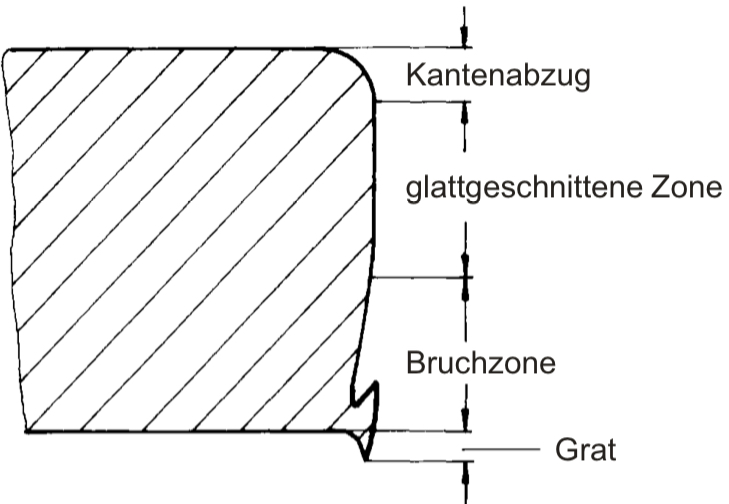
\includegraphics[width=0.8\linewidth]{src/images/Stanzen.jpeg}\\
\textbf{Verfahren:}\\
Aufsetzen des Stempels auf dem Blech, Plasitsche Verformung des
Werkstoffs, Rissbildung, Durchreissen.\\

\textbf{Feinschneiden:}\\
Beim Feinschneiden wird das Blech besonders gut eingespannt, 
sodass die Schnittkante rechtwinklig zur Planfläche des Werkstücks 
liegt.\\
Vorteile: hoher Rationalisierungsgrad, minimaler Kanterverzugs, glatte und abrissfreie Schnittfläche.\\
Schmale Rand- und Stegbreiten sind möglich. Fürs Feinschneiden ist eine gewisse Rauheit der Oberflächen nötig, um viel Reibung und genügend Halt zu gewährleisten. \\

\textbf{Masse:}\\
Beim Lochen (Innenformen) ist der Lochstempel bestimmend 
und erhält das Sollmass der Schnittteils.\\
Beim Ausschneiden 
(Aussenformen) ist der Scheidplattendurchbruch bestimmend und 
erhält das Sollmass des Schnittteils.\\
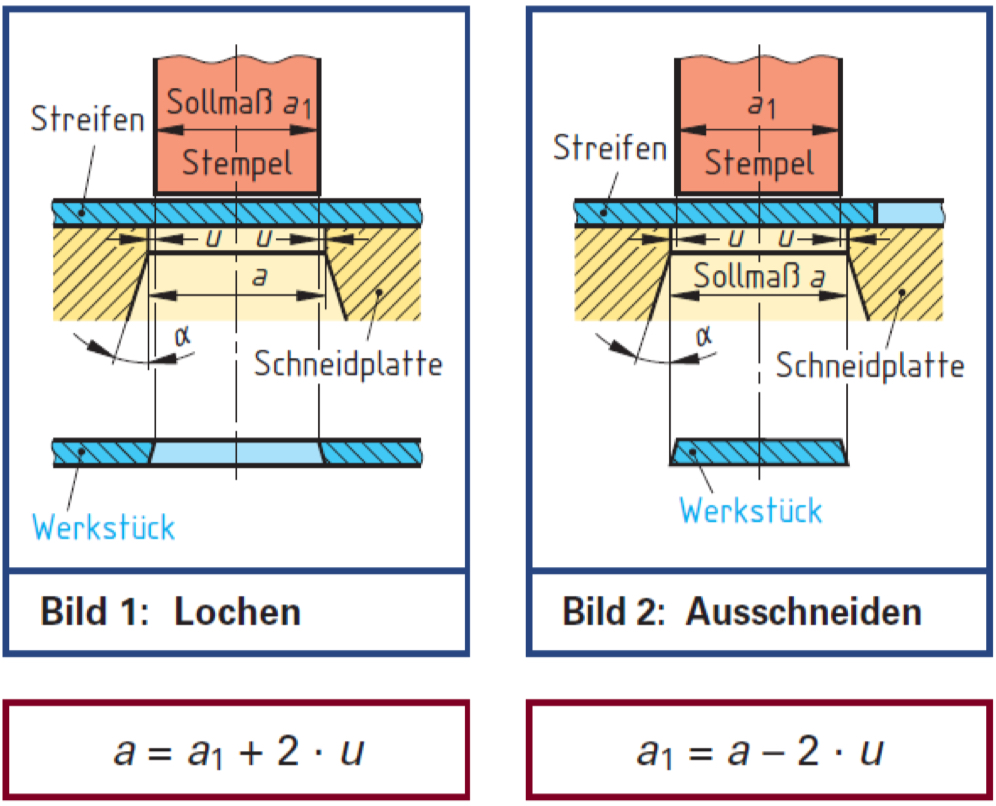
\includegraphics[width=\linewidth]{src/images/Masse Stanzen.jpeg}

    \subsubsection*{Spanen}
    Überschüssiges Material wird mit Werkzeugschneiden mechanisch abgetrennt. Dabei entstehen Späne.\\

Die wichtigsten zerspanenden Verfahren sind:
\begin{itemize}
    \item Drehen
    \item Bohren
    \item Fräsen
    \item Schleifen
\end{itemize}

\textbf{Geometrisch bestimmt:} \hfill (Drehen, Bohren, Fräsen)\\
Schneidkeil dringt in Werkstoff ein, elastische und plastische 
Verformung, Fliessen des Werkstoffes, Ausbildung eines Spans, 
Ablaufen des Spans über den Schneidkeil.\\

\textbf{Voraussetzungen:} hohe Härte des Werkzeugs und eine minimale Eindringtiefe.\\
Höhere Produktivität aber auch höhere Ungenauigkeit.\\
Rauheit 3. Ordnung, $R_z > 2.5 \mu m$\\

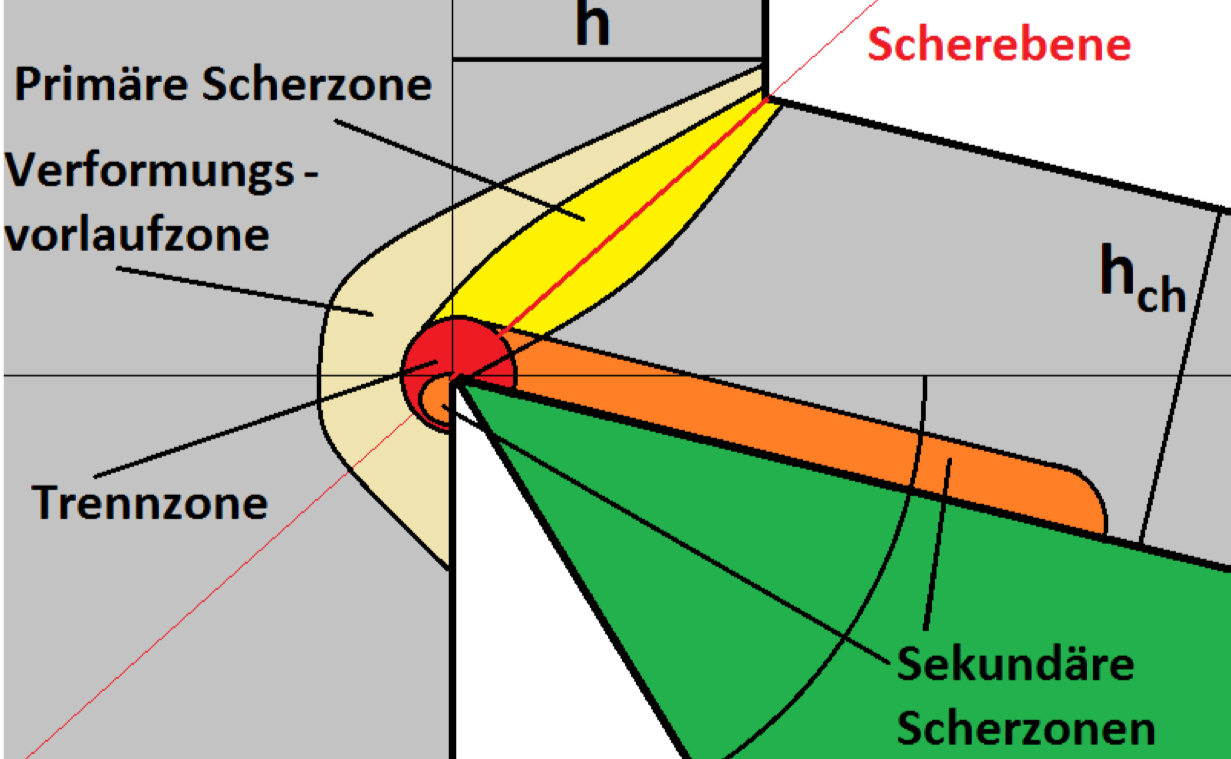
\includegraphics[width=0.8\linewidth]{src/images/Spanen.jpeg}\\
\textbf{Geometrisch Unbestimmt:} \hfill (Schleifen)\\
Abrasivkörner dringen in Wekrstoff ein, elastische und plastische 
Verformung, duktile Werkstoffe fliessen und bilden Mikro-Späne, 
Spröde Werkstoffe bilden Risse und Brechen aus. \\

\textbf{Voraussetzungen:} hohe Härte der Abrasivkörner sowie eine minimale Eindringtiefe.\\
Geringere Produktivität aber mehr Genauigkeit.\\
Eine grosse Porosität gibt Raum für die Späne und dient der Kühlung. \\
Rauheit 5.-6. Ordnung, $R_z < 2.5 \mu m$\\
    \subsubsection*{Drehen}
    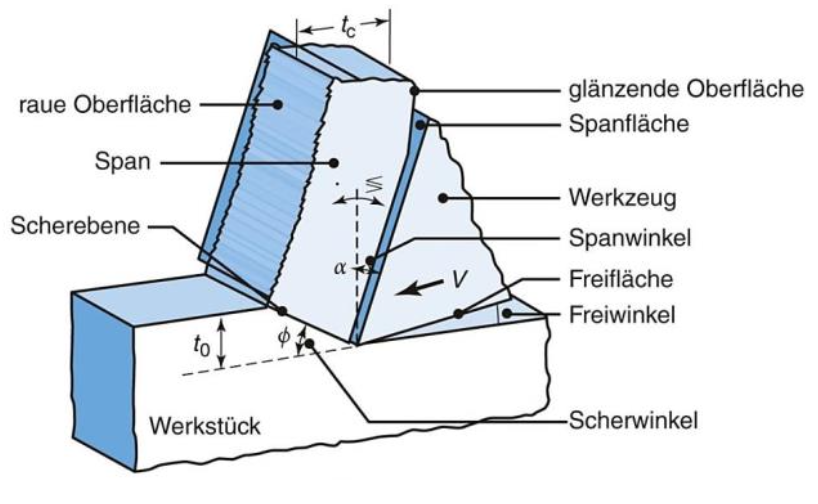
\includegraphics[width=35mm]{src/images/Zerspanvorgang1.png}
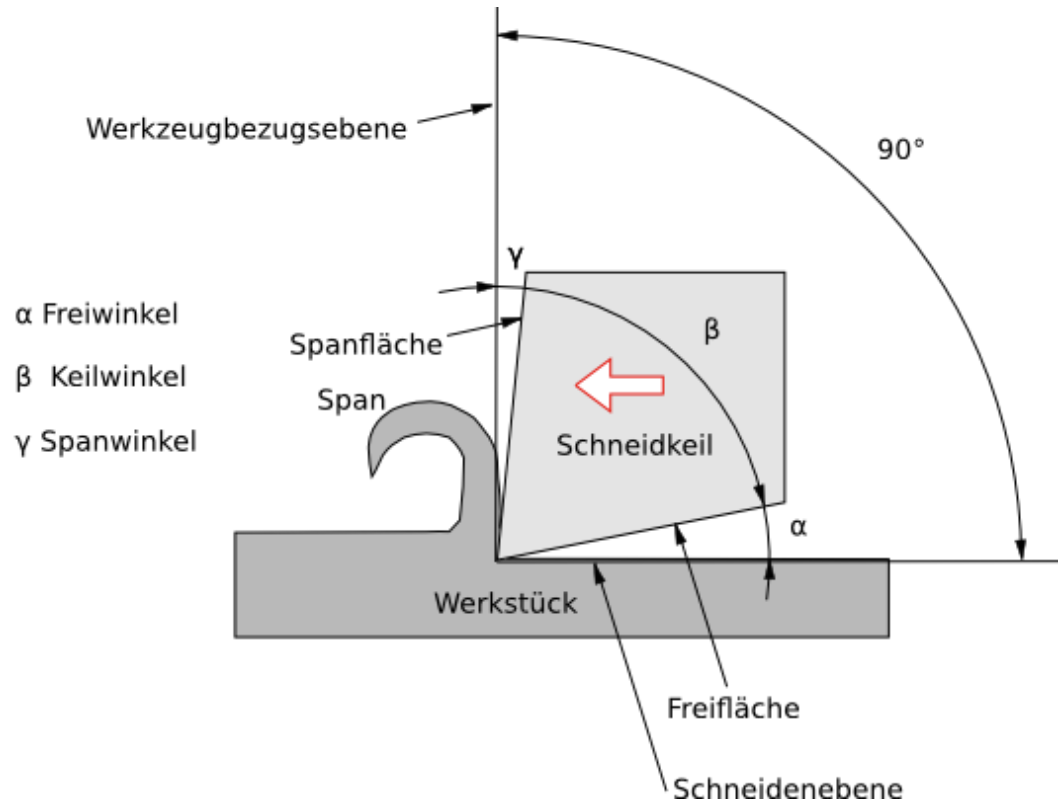
\includegraphics[width= 35mm]{src/images/Zerspanvorgang2.png}\\
\textbf{Verfahren:}\\
Spanen mit geschlossener, meist Kreisförmiger Schnittbewegung 
und beliebiger, quer zur Schnittrichtung liegender Vorschubachse. 
Die Drehachse behält ihre Lage zum Werkstück unabhängig von 
der Vorschubachse bei. \\

\textbf{Kinematische Rauheit, Schnittwinkrl – Drehen:}\\

\begin{minipage}{0.48\linewidth}
    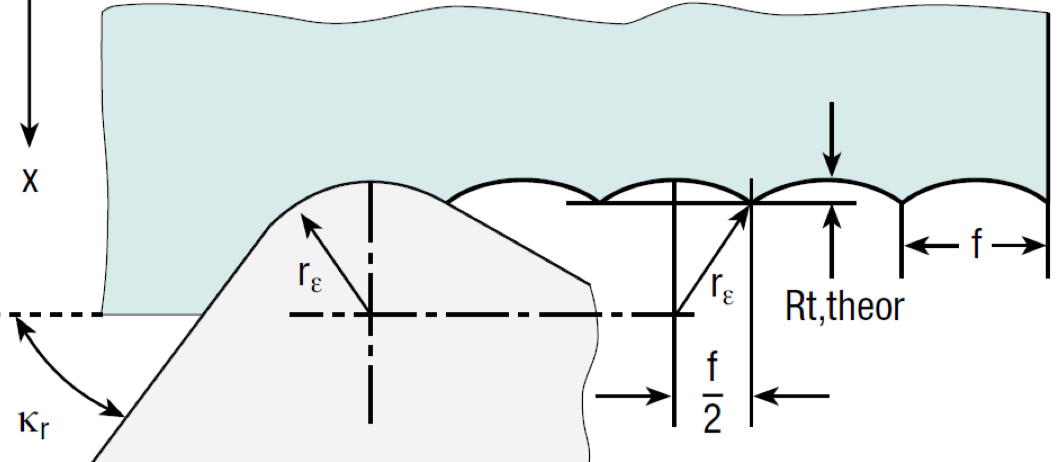
\includegraphics[width=35mm]{src/images/Kinematische Rauheit.jpeg}
    \begin{tiny}
    Theoretische Rauheit:\\ 
    \begin{center}
        \[
            \boxed{        
                R_{t,theor} = \frac{f^2}{8 r_{\varepsilon}}
                }
            \]
    \end{center}
    \end{tiny}
\end{minipage}
\begin{minipage}{0.48\linewidth}
    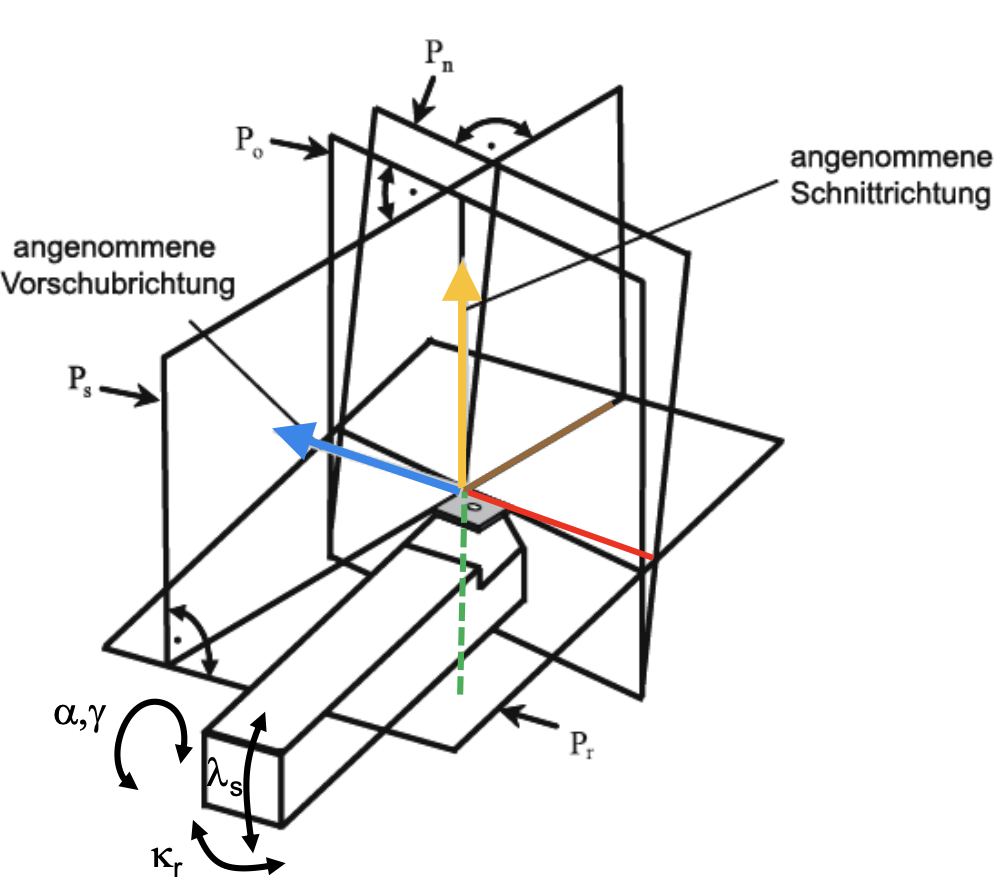
\includegraphics[width=35mm]{src/images/Winkel Drehen.png}\\
\end{minipage}
\\

\textbf{Winkel beim Drehen:}
\begin{itemize}
    \begin{tiny}
        \item Freiwinkel $\alpha$: Winkel zeischen Schneidebene und Freifläche (6°bis 12°)
        \item Keilwinkel $\beta$: Winkel zwischen Span- und Freifläche\\ ($\beta$ = 90 - $\alpha$ - $\gamma$)
        \item Spanwinkel $\gamma$: Winkel zwischen Spanfläche und Werkzeugbezugsebene (-15° bis +25°)
        \item Einstellwinkel $\kappa_r$: Winkel zwischen Hauptschneide und Vorschubrichtung (45° is 110°)
        \item Eckenwinkel $\varepsilon_r$: Winkel zwischen Haupt- und Nebenschneide (35° bis 100°)
        \item Neigungswinkel $\lambda$: Winkel zwischen Hauptschneide und Werkzeugebene (-6° bis +6°)
    \end{tiny}
    \end{itemize}

\textbf{Einfluss des Einstellwinkels:}\\

\begin{minipage}{0.5\linewidth}
    \[
    \boxed{     
        \begin{aligned}
            b &=\frac{a_p}{sin(\kappa_r)}\\
            h &=f\cdot sin(\kappa_r)\\
            A &=a_p\cdot f=b\cdot h
        \end{aligned}
        }
    \]
\end{minipage}
\begin{minipage}{0.5\linewidth}
    \begin{tiny}
    \item $b$: Spanungsbreite
    \item $a_p$: Schnitttiefe
    \item $\kappa_r$: Einstellwinkel
    \item $h$: Spanungsdicke
    \item $f$: Vorschub
    \item $A$: Spanuungsquerschnitt
    \end{tiny}
\end{minipage}\\

\textbf{Ursachen} zur Bildung von \textbf{diskontionuierlichen Spänen:}\\
Spröder Werkstoff, sehr hohe oder niederige Schnitt-\\
geschwindigkeit, grosse Schnitttiefe, geringer Spanwinkel, eiernde (nicht steife) Werkzeugmaschine\\

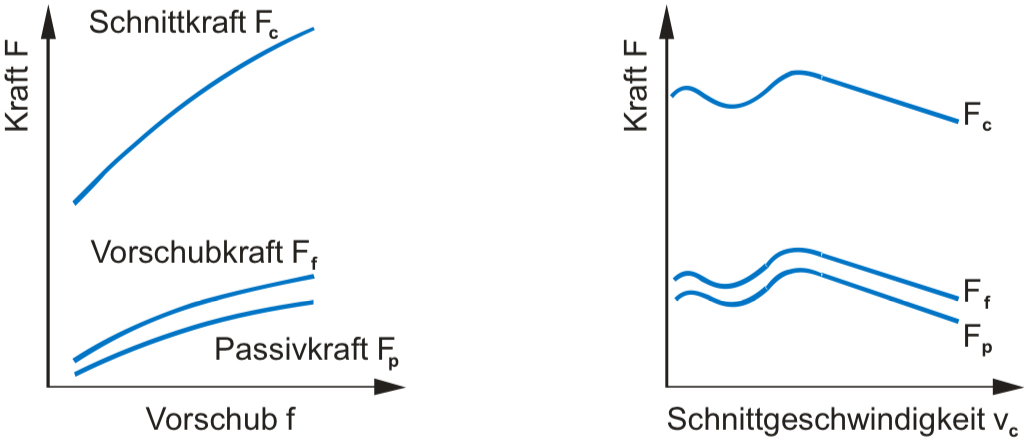
\includegraphics[width=35mm]{src/images/Trennen Diagramme1.jpeg}
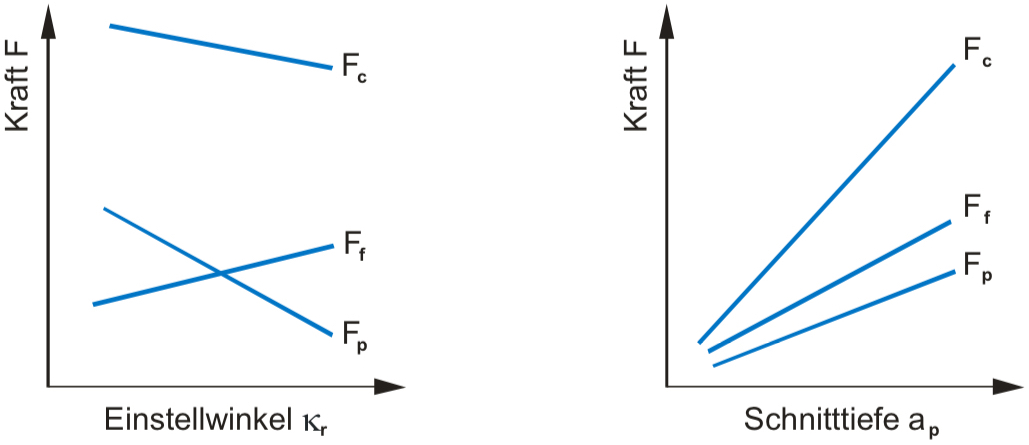
\includegraphics[width=35mm]{src/images/Trennen Diagramme2.jpeg}\\


    \subsection{Fräsen}
    \input{src/8_Trennen/Fräsen.tex}
    \subsection*{Verschleiss von Werkzeugen}
    \textbf{Adhäsion:} Ist bestimmt durch stoffliche Wechselwirkungen, durch lokale Pressungen an einzelnen Rauheitshügeln, es entstehen Kaltverschweissungen.\\

\textbf{Abrasion:}\\

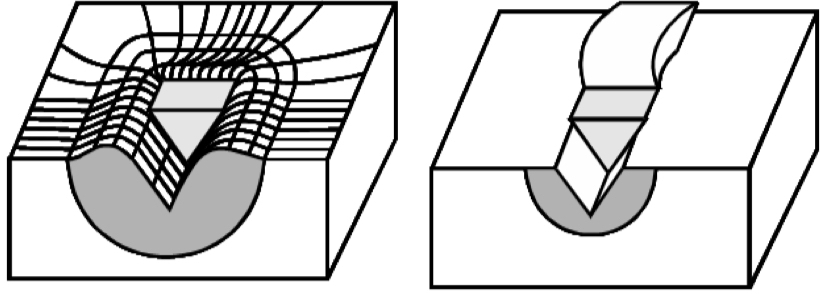
\includegraphics[width=0.5 \linewidth]{src/images/Verschleiss1.jpeg}
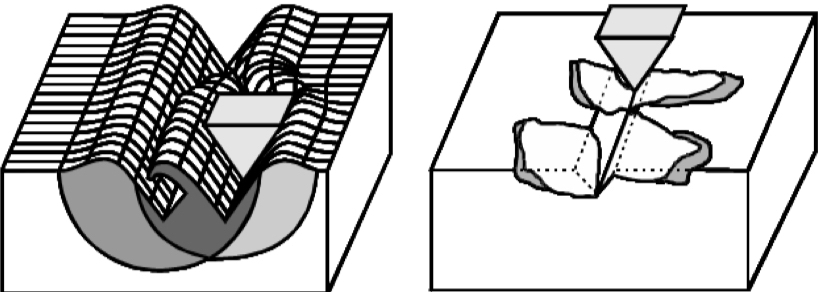
\includegraphics[width=0.5 \linewidth]{src/images/Verschleiss2.jpeg}

Mikropflügen, Mirkrospanen, Mirkoermüden, Mikrobrechen\\


\begin{minipage}{0.5\linewidth}
    \textbf{Verschleiss nach Archard:}\\
    \[
    \boxed{     
        V = k \frac{LF}{3H}
    }
    \]
\end{minipage}
\begin{minipage}{0.5\linewidth}
    \begin{tiny}
    \item $V$: Verschleissvolumen
    \item $k$: Verschleisskoeff.
    \item $L$: Gleitstrecke
    \item $F$: Normalkraft
    \item $H$: Härte
    \end{tiny}
\end{minipage}
\vspace{1mm}

\textbf{Standzeit nach Taylor:}\\
\begin{minipage}{0.5\linewidth}
    \[
    \boxed{     
        T_c = C_v \cdot v_c^k
    }
    \]
\end{minipage}
\begin{minipage}{0.5\linewidth}
    \begin{tiny}
    \item $T_c$: Standzeit
    \item $v_c$: Schnittgeschiwndigkeit
    \item $C_v$ und $k$: Werkzeugspez. Konstante
    \end{tiny}
\end{minipage}\\
\vspace{1mm}
\textbf{Kienze-Gleichung:}\\
\begin{minipage}{0.5\linewidth}
    \[
    \boxed{     
        F_s = \frac{F_c}{b}
    }
    \]
\end{minipage}
\begin{minipage}{0.5\linewidth}
    \begin{tiny}
    \item $F_s$: Spankraft
    \item $F_c$: Schnittkraft
    \item $b$: Schnittbreite/Spanungsbreite
    \end{tiny}
\end{minipage}\\
\vspace{1mm}

\textbf{Stumpfe Werkzeugspitze: }\\
$\uparrow$ Spitzenradius $r_t$ $\not\rightarrow$ $\downarrow$ Schnitttiefe, $\rightarrow$ $\uparrow$ Schnittkraft\\
$\uparrow$ Oberflächenspannung, Risse\\
$\uparrow$ Neigung der Aufbauschneidenbildung




\section*{Fügen}
    Fügen ist das auf Dauer angelegte Verbinden von Werkstücken mit 
geometrisch bestimmter Form.Verfahren sind dabei Punktscheissen, 
Laserschweissen, Stanznieten, Clinchen oder Kleben.\\

\textbf{Verbindungsarten:} 
\begin{itemize}
    \item Formschlüssig (Passfeder, Keilwelle, Passschraube, Stift, Bolzen, Nieten)
    \item Vorgespannt formschlüssig (Keil, Stirnzahn, Kegel mit Scheibenfeder)
    \item Kraftschlüssig (Schrauben, Klemmen, Kegelverbindung, Einscheibenkupplung)
    \item Stoffschlüssig (Schweissen, Löten, Kleben)
\end{itemize}

    \subsection*{Schweissen}
    \textbf{Definition:} Das Schweissen ist das schmelzflüssige Vereinigen 
von Werkstoffen in der Schweisszone unter Anwendung von Wärme 
und/oder Kraft mit oder ohne Schweisszusatz.\\

\begin{minipage}{0.5\linewidth}
    \begin{center}
        \textbf{WIG}
    \end{center}
    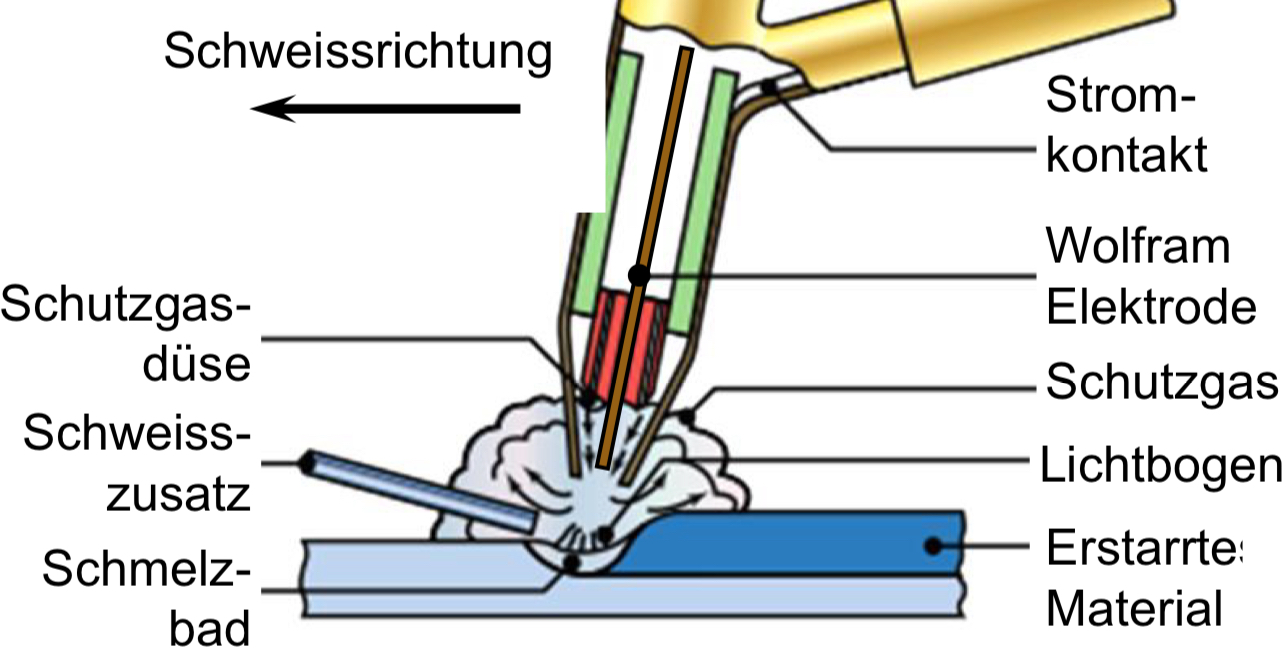
\includegraphics[width=\linewidth]{src/images/WIG.jpeg}\\
\end{minipage}
\begin{minipage}{0.5\linewidth}
    \begin{center}
        \textbf{MSG}
    \end{center}
    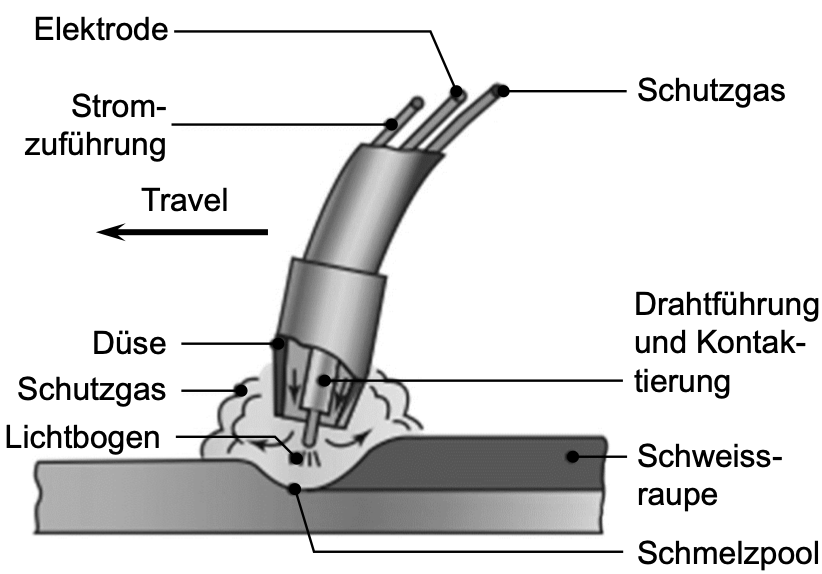
\includegraphics[width=\linewidth]{src/images/MSG.png}\\
\end{minipage}
\textbf{WIG:} Verwendet einen Gleichstromlichtbogen. 
Wolframelektrode hat negative Polarität und fungiert als Kathode. 
Das Werkstück ist die Anode. \\

\textbf{MSG (MIG/MAG) Schweissen:} Bei niedriger Spannung und Strommstärke 
treten Spritzer auf. Es wird kontrolliert zwischen globularem Materialübergang 
und Sprühtransfer gewechselt, um einzelne Tropfen zu übertragen. \\

\textbf{Plasmaschweissen:}\\
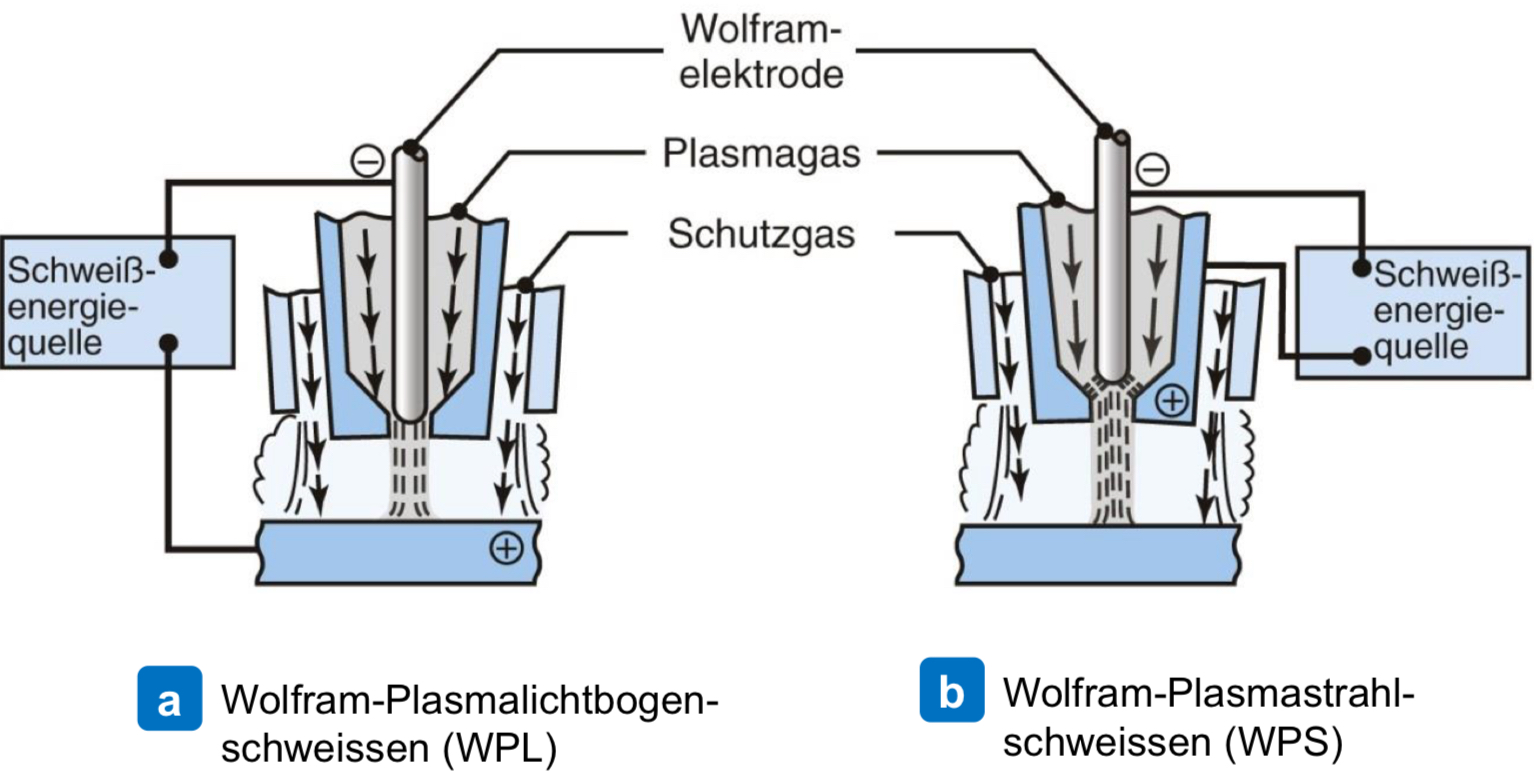
\includegraphics[width=0.8\linewidth]{src/images/WP.jpeg}\\

\textbf{Cold Metal Transfer (CMT):} Draht wird mit 50-130 Hz hin und 
her bewegt. CMT erkennt einen Kurzschluss und zieht Draht zurück. 
Vorteile sind kontrollierte und spritzerfreie Materialablagerung, 
geringe Wärmeeinwirkung und gute Energieeffizienz.\\

\textbf{Gleich- und Wechselstromschweissen:} Beim Gleichstromschweissen 
und negativ gepolter Elektrode ergeben sich die längsten 
Elektrodenstandzeiten. Im Werkstück bildet sich eine Art Kegel. 
Beim Wechselstromschweissen fliessen die Elektronen vom Werkstück 
zur Elektrode und reissen dabei die hochschmelzende Oxidschicht auf. 
Im Werkstück bildet sich eine Art Erhebung.\\

\textbf{Impulsschweissen:} Strom wird in Impulse unterteilt, weniger Wärme ins Material\\
"gezielt zwischen
globularem Materialübergang und Sprühtransfer
gewechselt, um einzelne Tropfen zu übertragen" - whatever\\

\textbf{Auslegung Schweissnaht:}\\


\begin{minipage}{0.55\linewidth}
    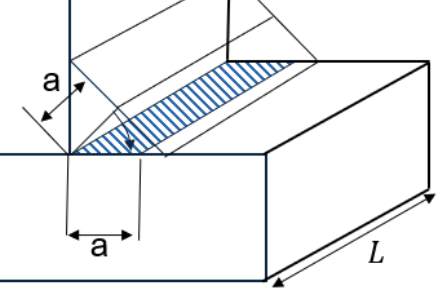
\includegraphics[width=0.8\linewidth]{src/images/Schweissnaht.png}\\
\end{minipage}
\begin{minipage}{0.30\linewidth}
    \[
        \boxed{     
            \begin{aligned}
                \sigma_{eq} &= \frac{F}{A_f}\\
                A_f &= l_{eff} \cdot a\\
                l_{eff} &= L - 2 \cdot a
            \end{aligned}
        }
        \]
\end{minipage}\\

\textbf{Reibschweissen:}\\
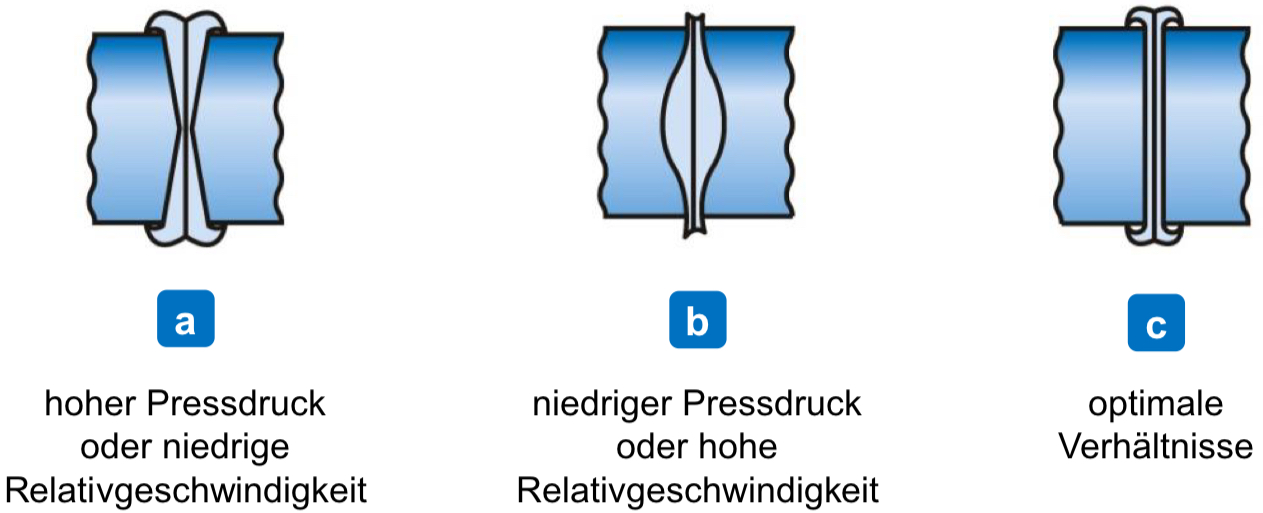
\includegraphics[width=\linewidth]{src/images/Reibschweissen.jpeg} \\

\textbf{Schweissnähte:} \\
Breite und Dicke der Schweissnaht nimmt mit der Drahtvorschubgeschwindigkeit zu.\\

\textbf{Schweissgeschwindigkeit:}\\
\begin{minipage}{0.5\linewidth}
    \[
    \boxed{     
        v_t = \frac{v_w \cdot A_{w}}{\textcolor{ForestGreen}{A_{b}}}
    }
    \]
\end{minipage}
\begin{minipage}{0.5\linewidth}
    \begin{tiny}
    \item $v_{t}$: Schweissgeschwindigkeit
    \item $v_w$: Drahtvorschubgeschwindigkeit
    \item $A_w$: Drahtquerschnitt
    \item $\textcolor{ForestGreen}{A_b}$: Raupenquerschnitt
    \item $\textcolor{red}{A_e}$: Einbrandzone
    \end{tiny}
\end{minipage}\\
\textbf{Schweissraupen:} Querschnittsform mit Parabel approximierbar.\\
Querschnittsfläche aus Kontinuitätsgleichung:\\

\textbf{Schutzgasschweissen Leistung Auslegung:}\\

\begin{minipage}{0.5\linewidth}
    \[
    \boxed{     
        \begin{aligned}
            P &= V \cdot I \cdot \eta \\
            &= V \cdot K \cdot v_{w} \cdot \eta
        \end{aligned}    
        }
    \]
\end{minipage}
\begin{minipage}{0.5\linewidth}
    \begin{tiny}
    \item $P$: Leistung beim Schweissen
    \item $V$: Spannung
    \item $I$: Strom
    \item $\eta$: Wirkungsgrad
    \item $K$: Proportionalitätsfaktor
    \end{tiny}
\end{minipage}\\
\vspace{1mm}


\textbf{Aufmischung D:} 
    \begin{tiny}
 \[
    \boxed{     
        D=\frac{\text{Zusatzmaterial}}{\text{Zusatzmaterial } + \text{ Grundmaterial}} = \frac{A_b}{\textcolor{ForestGreen}{A_b} + \textcolor{red}{A_e}}
    }
    \]
    \end{tiny}\\
Bsp. "80\% Aufmischung" bedeutet, dass 80\% vom Grundmaterial 
und 20\% vom Füllmaterial stammen.\\

\textbf{Schmelzbad:} 
\begin{itemize}
    \item \textbf{DC, Elektrode negativ:} \\Tiefes Schmelzbad, keine Oberflächenreinigung
    \item \textbf{DC, Elektrode positiv:} \\Seichtes Schmelzbad, Oberflächenreinigung
    \item \textbf{AC:} Intermediate
\end{itemize}

\textbf{Störungsfaktoren - Schmelzbad:} Auftrieb, Oberflächenspannung, Lorentzkraft, Scherspannung des Schutzgasstroms\\

\textbf{Fehler in Schweissnähten:} Längsrisse, Querrisse, Kerbrisse, 
Überlappungen, Einrandkerben, Einschlüsse, Porosität, Ungenügende 
Durchschweissung, Nahtunterschreitung, unvollständige Verbindungen. \\
Entstehen durch zu geringen Schutzgasfluss, instabile Keyholes, 
Kontamination der Oberflächen.\\
\includegraphics[width=0.5\linewidth]{src/images/Schäfflerdiagramm.png}\\

\textbf{Schäfflerdiagramm:} Das Schäfflerdiagramm kann die resultierende 
Phasenzusammensetzung eines Chrom-Nickel-Stahs abgeschätzt werden. 
Dabei berücksichtigt werden Ni, C, Mn, N, Mo, Si, Nb, Ti.\\






    \subsection*{Löten}
    \begin{itemize}
    \item Weichlöten (unterhalb 450°C, SnAg5, PbAg5, Au4Sn)
    \item Hartlöten (oberhalb 450°C, CuZn, AgCuZn, AlSi12)
    \item Hochtemperaturlöten (über 900°C)
\end{itemize}
Beim Löten ist es einfacher, zwei unterschieldicher Materialien zu 
verbinden als beim Schweissen. Ausserdem wird beim Löten immer 
ein Füllmaterial benötigt.

    \subsection*{Fügen durch Umformen}
    \begin{itemize}
    \item Clinchen (Verfalten von Blechen)
    \item Nieten
    \item Schnappverbinder
    \item Walzplattieren
    \item Rührreibschweissen
\end{itemize}
    \subsection*{Kleben}
    \textbf{Definition:} \\
Beim Kleben werden gleiche oder unterschieldiche 
Stoffe durch eine aushärtende Zwischenschicht stoffschlüssig 
und nicht lösbar verbunden. Die Klebewirkung beruht auf der 
\textbf{Adhäsionskraft des Klebstoffes an den Fügeflächen} und der 
\textbf{Kohäsionskraft im Innern der Klebeschicht}. Klestoffe können 
gut Scherkräfte aufnehmen.\\

\textbf{Vorteile:}\\
Keine Gefügeänderung, gleichmässige Spannungsverteilung, 
viele Werkstoffkombinationen, dichte Verbindungen, 
wenig Passarbeit nötig, grossflächige Verbindungen.\\

\textbf{Nachteile:}\\
grosse Fügeflächen nötig, geringe Festigkeit, geringe Temperaturbeständigkeit, 
lange und komplizierte Aushärtung, keine 
zerstörungsfreie Prüfung möglich, anfällig für Schälkräfte.\\

\textbf{Physikalisch abbindende Klebstoffe:}
\begin{itemize}
    \item Lösungsmittelklebstoffe härten durch Ablüften des 
    Lösungsmittels. Sie basieren auf gelösten Kautschuken.
    \item Schmelzklebstoffe härten durch Abkühlung
    \item Dispersionsklebstoffe benötigen. Wärmeeinwirkung zum 
    Aushärten. Sie basieren auf PVC, Weichmachern, Füllstoffen 
    und Haftvermittlern.
\end{itemize}

\textbf{Chemisch abbindende Klebstoffe:}
\begin{itemize}
    \item Polmerisationsklebstoffe werden katalytisch durch 
    Feuchtigkeit ausgelöst.
    \item Bei Polyadditionsklebstoffen reagieren mindestens zwei 
    unterschiedliche Stoffe miteinander verbunden.
    \item Polykondensationsklebstoffe reagieren unter der Abspaltung 
    von flüchtigen Stoffen. Benötigen Pressdruck von mindestens
     $40 N/cm$ und oft erhöhte Temperaturen.
\end{itemize}
    % \vfill \null \columnbreak




\end{document}